\documentclass[12pt, a4paper, openright, twoside]{report} % Use report or book for thesis style, default style was article
\usepackage{graphicx} % Required to import external graphics files
\graphicspath{ {./pics/} }
\usepackage[italian]{babel} % Set document language
\usepackage{xcolor} % Text color (use [dvipsnames] for additional colors, with different naming)
\usepackage{tabularx} % Tables with auto-sizing columns
\usepackage{multirow} % Tables with headers spanning multiple columns
\def\code#1{\texttt{#1}} % Monospace code font with a nicer name than the default texttt, which TBH just looks like a typo
\usepackage{float} % Makes you able to display a figure exactly where you place it, thanks to attribute [H]
\usepackage{enumitem} % Makes it possible to remove indentation from lists
\usepackage[utf8]{inputenc} % Set document encoding to UTF-8. You could also use \usepackage[T1]{fontenc}, but it would increase compile time
\definecolor{MaterialBlue}{HTML}{0843D8} % Material Design Blue, using it for hyperlinks
\usepackage{indentfirst} % Indent first line in chapters
\usepackage{titlesec}
\titleformat{\chapter}{}{}{0em}{\bf\Huge} % Remove "Chapter N" heading, leaving chapter title only at its default font size and style

\usepackage{fancyhdr}   % Set document
\usepackage{newlfont}   % Use specific fonts, such as \textsc{}

% Math libraries
\usepackage{amssymb}
\usepackage{amsmath} % Create matrices
\usepackage{latexsym}
\usepackage{amsthm}
\usepackage{cite}
\usepackage{listings}
\usepackage{hyperref} % Hyperlinks for websites
\usepackage[square, numbers, sort]{natbib}

\usepackage{fixltx2e}   % Subscript text
\usepackage{fancyvrb}	% For "\Verb" macro
\usepackage[normalem]{ulem}	% Strikethrough text

\oddsidemargin = 30pt % Vertical margin
\evensidemargin = 20pt % Horizontal margin

\linespread{1.3} % Set line height

\lstset{
	frame=single,
	breaklines=true
}

\hyphenation{sil-la-ba-zio-ne pa-ren-te-si} % Hyphenation within parentheses: insert each word that LaTeX can't break correctly into a newline

% Page setup using fancyhdr library
\pagestyle{fancy}\addtolength{\headwidth}{20pt}
\renewcommand{\chaptermark}[1]{\markboth{\thechapter.\ #1}{}}
\renewcommand{\sectionmark}[1]{\markright{\thesection \ #1}{}}
\rhead[\fancyplain{}{\bfseries\leftmark}]{\fancyplain{}{\bfseries\thepage}}
\cfoot{}

% \maketitle

\newcommand{\xsupervisor}{Giovanni Delnevo}
\newcommand{\xcorrelatore}{Kelvin Olaiya}
\newcommand{\xstudent}{Francesco Valentini}


\begin{document}

% Choose page size
%\setlength{\textwidth}{13.5cm}
%\setlength{\textheight}{19cm}
%\setlength{\footskip}{3cm}

\oddsidemargin = 25pt

\begin{titlepage}
    \begin{center}
    {
        {\Large{\textsc{Alma Mater Studiorum}}} \\
        {\Large{\textsc{Università di Bologna}}} \\
        {\textsc{Campus di Cesena}}
        \vspace{-1mm}
    }
    \end{center}
    \begin{center}
    {
        % Rule width was formerly 14cm: a bit too large for this page
        \rule[0.1cm]{\textwidth}{0.1mm}
        \rule[0.5cm]{\textwidth}{0.6mm}
        DIPARTIMENTO DI INFORMATICA - SCIENZA E INGEGNERIA
        Corso di Laurea in Ingegneria e Scienze Informatiche
    }
    \end{center}

    \vspace{2.25cm} % Formerly 15mm, then became 25mm, then 3.236cm

    \begin{center}
        {\LARGE{\textbf{LOREM IPSUM}}} \\
        \vspace{0.4cm}
        {\LARGE{\textbf{DOLOR SIT AMET}}} \\
        \vspace{0.4cm}
        {\LARGE{\textbf{EXPECTO TITOLORUM}}} \\
        \vspace{0.4cm}
        {\LARGE{\textbf{(TODO: alla fine)}}}
    \end{center}

    \vspace{2.25cm} % Formerly 40mm, then became 30mm, then 3.236cm
    \par
    \noindent
    \begin{minipage}[t]{0.47\textwidth}
        {\large{\textbf{Relatore:}}} \\
        {\large{\textbf{Prof. \xsupervisor}}}
        % \vspace{0mm}
        % \hfill
        % {\large{\bf \\Correlatore:\\
        % Dr. \xcorrelatore}}
    \end{minipage}
    % \vspace{1cm}
    % \par
    % \noindent
    \hfill
    \begin{minipage}[t]{0.47\textwidth}\raggedleft
        {\large{\textbf{Presentata da:} \\
        {\large{\textbf{\xstudent}}}}}
    \end{minipage}
    % \begin{center}
    %     {\large{\textbf{\xstudent}}} \\
    %     \vspace{1mm}
    %     {\large{\textbf{Matr. \xstudentid}}}
    % \end{center}

    % \begin{flushright}
    %     \begin{minipage}
    %         {0.47\textwidth}
    %         \raggedleft
    %         \vspace{-2mm}
    %         {\large{\textbf{Matricola n° \xstudentid}}}
    %     \end{minipage}
    % \end{flushright}

    \vspace{1cm}

    \begin{center}
        {\large{\textbf{Sessione IV\\Anno Accademico 2023/2024}}}
    \end{center}
\end{titlepage}

\begin{titlepage}
\thispagestyle{empty}
\topmargin=6.5cm
\raggedleft
\large
\em
% Questa \`e la \textsc{Dedica}:\\
% ognuno pu\`o scrivere quello che vuole, \\
% anche nulla \ldots                      %\ldots lascia tre puntini

To the moments we never expected,\\
\vspace{1.4mm}
and the trails that time had connected.\\   % connected, directed, perfected
\vspace{1.4mm}
To the friends and family found along the way,\\
\vspace{1.4mm}
and my sister Anna, whose light will forever stay.
\newpage



\clearpage{\pagestyle{empty}\cleardoublepage}
\end{titlepage}
\pagenumbering{roman}
\chapter*{Introduzione}
\addcontentsline{toc}{chapter}{Introduzione}

TODO

\newpage

% Set page header
\rhead[\fancyplain{}{\bfseries\leftmark}]{\fancyplain{}{\bfseries\thepage}}
\lhead[\fancyplain{}{\bfseries\thepage}]{\fancyplain{}{\bfseries
INDICE}}
\tableofcontents    % Create index of contents
% \newpage
% No numbering on last page on left side
\clearpage{\pagestyle{empty}\cleardoublepage}
\listoffigures  % Create index of figures
% \newpage
% No numbering on last page on left side
\clearpage{\pagestyle{empty}\cleardoublepage}
\listoftables   % List of tables
% \newpage

\clearpage{\pagestyle{empty}\cleardoublepage}
\chapter{Contesto}
\lhead[\fancyplain{}{\bfseries\thepage}]{\fancyplain{}{\bfseries\rightmark}}
\pagenumbering{arabic}

In questo capitolo andremo a esplorare alcune delle tecnologie emergenti nel settore digitale che stanno inesorabilmente trasformando il mondo che ci circonda, lasciando un deciso impatto sulla realtà. Vedremo i soggetti chiave di questo cambiamento, sia a livello globale parlando di \textit{Open Data} in generale, sia trattando gli impatti che questi ultimi stanno lasciando a livello locale sul nostro territorio, con progetti come \textit{BolognaWiFi} del Comune di Bologna. Quindi, solleveremo la questione di come questi dati possano essere visualizzati per riuscire a trarne il maggior beneficio, e infine analizzeremo gli impatti di queste iniziative sulla realtà, considerandone sia le sfide che le opportunità offerte.
Approfondiremo in sequenza ciascuna di queste sezioni, per riuscire ad avere una comprensione completa di come queste tecnologie stanno lasciando un impatto sulle nostre città.
% TODO: descrizione di una pagina sugli argomenti che andremo a trattare in questo capitolo \newpage

\section{Open Data} % : definizione e contesto
Le nuove tecnologie permettono di creare servizi in grado di migliorare la vita dei cittadini e di far funzionare più efficientemente governi e società. Molti dei dati necessari a raggiungere questi obiettivi sono prodotti da organismi pubblici, tuttavia spesso tali dati non sono disponibili in formati che li rendano facili da manipolare. Per questo motivo, da diversi anni si utilizza la nozione di \textit{open data}, i cosiddetti dati aperti, e più specificamente gli \textit{open government data}, ovvero quelli riguardanti il settore pubblico del governo, intesi come informazione, pubblica o privata, accessibile e riutilizzabile da chiunque e per qualsiasi fine.

Come possiamo vedere in Figura~\ref{fig:open_data_google_trends}, questo termine entra nell'uso comune a partire dal 2009, quando diversi governi hanno annunciato nuove iniziative per l'apertura della loro informazione pubblica, tra cui quelli di Stati Uniti, Regno Unito, Canada e Nuova Zelanda \cite{OpenDataHandbook_Introduction}.

\begin{figure}[H]
    \centering
    \includegraphics[width=\textwidth]{open_data_google_trends}
    \caption[Open Data su Google Trends]{Ricerche su Google relative al termine Open Data effettuate dal 2004 al 2025. Notare l'aumento successivo al 2009 e il trend in crescita \cite{Google_Trends}.}
    \label{fig:open_data_google_trends}
\end{figure}

\subsection{Concetto di Open Data}
%Definizione e principi fondamentali
Gli \textit{open data}, specialmente quelli della pubblica amministrazione, costituiscono una formidabile risorsa che ancora oggi rimane in larga parte inutilizzata. Molte persone e organizzazioni raccolgono una vasta gamma di svariati tipi di dati per svolgere le proprie attività. In questo ambito, il governo riveste particolare importanza, sia per la quantità e la centralità dei dati che raccoglie, sia perché la maggior parte dei dati del governo sono pubblici per legge, quindi potrebbero diventare aperti e resi disponibili per l'utilizzo da parte di chiunque. Questo riveste particolare interesse in quanto si ritiene che gli \textit{open data} possano apportare benefici in molti settori, ed esistono altrettanti esempi di come siano già stati usati con successo. Ci sono inoltre svariati gruppi di persone e organizzazioni che possono trarre vantaggi dalla disponibilità di \textit{open data}, incluso il governo stesso. Allo stesso tempo, è impossibile effettuare previsioni esatte su come e dove verranno apportati questi benefici in futuro, perché per natura dell'innovazione gli sviluppi partono spesso dai posti più inaspettati \cite{OpenDataHandbook_WhyOpenData}.

\subsection{Caratteristiche principali degli Open Data}
% Accessibilità, Interoperabilità, Riutilizzabilità
% Formati comuni: CSV, JSON, XML
In base a quanto stabilito dalla \textit{Open Definition}, gli \textit{open data} sono dati che possono essere utilizzati liberamente e ridistribuiti da chiunque e sono sottoposti, al massimo, al riconoscimento obbligatorio di una potenziale attribuzione o crediti in generale \cite{OpenDefinition}. 

Nella \textit{full Open Definition} vengono specificate in dettaglio le proprietà più importanti, ovvero:

\begin{itemize}
    \item \textbf{Disponibilità e accesso}\\
    I dati devono essere disponibili per intero, senza pagare più di un costo ragionevole di riproduzione, preferibilmente scaricandoli dalla rete Internet. I dati devono, inoltre, essere disponibili in un formato conveniente e modificabile.
    \item \textbf{Riutilizzo e ridistribuzione}\\
    I dati devono essere forniti sotto licenza che ne permetta liberamente il riutilizzo e la ridistribuzione, incluso specialmente il mescolamento con altri \textit{dataset}.
    \item \textbf{Partecipazione universale}\\
    Tutti devono essere in grado di utilizzare, riutilizzare e ridistribuire i dati, senza discriminazioni contro campi di applicazione o contro persone o gruppi particolari. Ad esempio, non sono permesse le licenze ristrette ai soli scopi non-commerciali, che impedirebbero l'utilizzo commerciale, e nemmeno qualsiasi altra restrizione all'uso per certe finalità, come quella esclusivamente educativa.
\end{itemize}

Queste regole sono necessarie per garantire chiarezza sul significato di apertura e, soprattutto, per assicurarne l'\textit{interoperabilità}. Quest'ultima denota la capacità di lavorare insieme, ovvero interoperare, tra diversi sistemi e organizzazioni, che in questo caso si riferisce all'interoperabilità, detta anche mescolanza, tra dataset differenti. \`E una capacità molto importante perché permette a diversi componenti di collegarsi per lavorare insieme e questo è essenziale per realizzare sistemi grandi e complessi, la cui costruzione altrimenti sarebbe quasi impossibile senza interoperabilità \cite{OpenDefinition_Full}.

Il principio cardine di un \textit{commons} di dati o codice, ovvero una raccolta di essi, è che un qualunque pezzo di materiale aperto lì contenuto possa essere mescolato liberamente con altro materiale aperto. Questa interoperabilità è assolutamente necessaria a livello pratico per realizzare i principali benefici ottenibili dall'apertura dei dati, ovvero l'abilità notevolmente migliorata di combinare insieme diversi dataset e di conseguenza la capacità di sviluppare un numero maggiore di prodotti e servizi aventi qualità migliore. Questa definizione data riguardo all'apertura assicura che, dati due dataset aperti ottenuti da due fonti diverse, possiamo essere sempre in grado di combinarli insieme, evitando di trovarci di fronte a un numero enorme di dataset aventi scarsa o nulla capacità di essere mescolati insieme in sistemi di più larga scala, senza quindi avere la capacità di apportare valore aggiunto. Il punto chiave di aprire i dati deve essere il \textit{focus} su dati non-personali, ovvero i dati non devono contenere informazioni riguardanti persone specifiche. Inoltre, per alcuni tipi di dati ottenuti dal governo, potrebbero applicarsi restrizioni nazionali per motivi di sicurezza \cite{OpenDataHandbook_WhyOpenData}.

\subsection{Formati principali}
Gli open data possono essere utilizzati in svariati formati, di seguito vediamo quali.
\subsubsection{JSON}
Quello più utilizzato in ambito software è JSON, un semplice formato file che è molto facile da leggere per qualsiasi linguaggio di programmazione. La sua semplicità lo rende più veloce da processare per un computer rispetto ad altri formati come XML.
\subsubsection{XML}
XML è un formato molto utilizzato per lo scambio di dati, in quanto fornisce buone opportunità di mantenere la struttura dei dati e il modo in cui i file sono costruiti, permettendo agli sviluppatori di scrivere parti della documentazione insieme ai dati senza interferire con la loro lettura.
\subsubsection{RDF}
RDF è un formato raccomandato dal W3C e rende possibile rappresentare i dati in una forma in cui sono più facili da combinare con altri dati provenienti da più fonti. Dati RDF possono essere salvati in varie serializzazioni, tra cui XML e JSON. RDF incoraggia l'utilizzo di URL come identificatori, fornendo un modo conveniente di interconnettere direttamente iniziative open data già esistenti sul Web. Non è ancora molto diffuso, ma è diventato un trend tra le iniziative di Open Government, tra cui annoveriamo i progetti di Open Data collegati tra i governi di Regno Unito e Spagna. L'inventore di Internet, Tim Berners-Lee, ha recentemente proposto uno schema chiamato \textit{fivesstar} che include i dati RDF collegati, ponendolo come obiettivo da raggiungere per le iniziative di open data.
\subsubsection{\textit{Spreadsheet}}
Sono utilizzati da molte autorità, le quali hanno ancora delle informazioni rimaste in documenti come quelli di Microsoft Excel. Questi dati possono essere utilizzati immediatamente con la corretta descrizione del significato delle varie colonne. Tuttavia, in alcuni casi ci possono essere delle macro e delle formule nei fogli di calcolo, che possono diventare potenzialmente più complicate da gestire. Di conseguenza, è consigliabile documentare questo genere di calcoli di fianco allo \textit{spreadsheet}, dato che è generalmente più accessibile alla lettura da parte degli utenti.
\subsubsection{\textit{Comma-Separated Values}}
I file CSV possono essere un formato molto utile data la loro compattezza e possono quindi essere adatti al trasferimento di grandi quantità di dati all'interno della stessa struttura. Tuttavia, questo formato è talmente spartano che i dati sono spesso inutili senza appropriata documentazione, dato che può essere quasi impossibile indovinare il significato delle diverse colonne. Diventa quindi particolarmente importante che la documentazione dei singoli campi sia accurata. Inoltre, è essenziale rispettare la struttura del file, in quanto la singola omissione di un campo è in grado di disturbare la lettura di tutti i rimanenti dati del file senza avere una reale opportunità di aggiustamento, perché non si può determinare come vanno interpretati i dati rimanenti.
\subsubsection{Documento di testo}
I documenti classici in formati come Word, ODF, OOXML o PDF potrebbero bastare per mostrare alcuni tipi di dati, come delle \textit{mailing lists} relativamente stabili o equivalenti, senza richiedere un grande sforzo. Questo formato non offre alcun supporto per il mantenimento di una struttura coerente, il che spesso significa che diventa difficile inserire dati mediante strumenti automatizzati. Bisogna assicurarsi di utilizzare dei \textit{templates} come base dei documenti che mostreranno dati per il riuso, così da rendere possibile ottenere informazioni da tali documenti. Inoltre, per supportare ulteriormente l'utilizzo dei dati si potrebbero utilizzare dei \textit{markers} tipografici il più possibile, così da rendere più facile per una macchina la distinzione degli \textit{headings}, ovvero i titoli di qualsiasi tipo, dal contenuto, e così via. Generalmente è raccomandabile non esibirli in un formato di \textit{word processing}, se i dati esistono in formati differenti.
\subsubsection{Testo non formattato}
I documenti di testo non formattato (.txt) sono molto semplici da leggere per un computer, ma generalmente escludono metadati strutturali dall'interno del documento, quindi gli sviluppatori devono creare un \textit{parser} che possa interpretare ogni documento nell'ordine in cui appare. Possono verificarsi alcuni problemi dallo scambio di file \textit{plain text} tra diversi sistemi operativi, in quanto Windows, macOS e altre varianti Unix hanno ciascuno il loro modo di indicare al computer che si è raggiunta la fine della riga, quindi 3 diversi caratteri di \textit{newline}.
\subsubsection{Immagini scannerizzate}
Probabilmente questo è il metodo meno indicabile per la maggioranza dei dati, ma sia TIFF che JPEG-2000 sono in grado di dargli una documentazione di ciò che si trova nell'immagine, e possono addirittura indicare testualmente l'intero contenuto del documento all'interno di un'immagine dello stesso documento. Potrebbe essere rilevante mostrare dati come immagini i cui dati non sono stati creati elettronicamente, un esempio sono i materiali di archivio, per i quali avere un'immagine è sicuramente meglio di nulla.
\subsubsection{Formati proprietari}
Alcuni sistemi dedicati hanno i propri formati di dati con cui possono essere salvati o esportati. Talvolta può bastare esporre i dati in tale formato, specialmente se ci si aspetta che un ulteriore utilizzo avvenga in un sistema simile a quello da cui provengono. Va sempre indicato dove si possono trovare ulteriori informazioni su questi formati proprietari, per esempio fornendo un link al sito web del fornitore. Generalmente, se fattibile, è raccommandabile mostrare i dati in formati non-proprietari.
\subsubsection{HTML}
Al giorno d'oggi, molti dati sono disponibili in formato HTML su vari siti e questo potrebbe tranquillamente essere sufficiente se i dati sono molto stabili e con ambito limitato. In alcuni casi, però, potrebbe essere preferibile avere i dati in una forma più facile da scaricare e manipolare, ma dato che il riferimento a una pagina su un sito web è una modalità molto semplice ed economica, potrebbe costituire un buon punto di partenza nella visualizzazione di dati. Tipicamente, sarebbe più appropriato utilizzare delle tabelle in documenti HTML per contenere i dati, ed è importante che i vari campi di dati siano visualizzati e assegnati degli ID che li rendano facili da trovare e manipolare i loro dati. Per effettuare lo scraping, Yahoo ha sviluppato un \textit{tool} in grado di estrarre informazioni strutturate da un sito, e tali strumenti sono in grado di effettuare molte altre operazioni purché i dati siano accuratamente etichettati \cite{YahooDevelopers_YQL}.

% \subsection{Confronto con dati privati}
% Differenze principali

% Vantaggi e svantaggi rispetto agli Open Data

\subsection{Contesto di applicazione}
Ad oggi, è già possibile indicare un cospicuo numero di settori nei quali i dati aperti del governo stanno già apportando un certo valore, tra cui:

\begin{itemize}
    \item Controllo di trasparenza e democrazia.
    \item Partecipazione.
    \item Autopotenziamento.
    \item Miglioramento o creazione di nuovi prodotti e servizi da parte di privati.
    \item Innovazione.
    \item Miglioramento dell'efficienza di servizi del governo.
    \item Miglioramento dell'efficacia di servizi governativi.
    \item Misuramento dell'impatto di certe politiche.
    \item Nuova conoscenza ottenuta dalla combinazione di fonti di dati e dalla ricerca di \textit{pattern} all'interno di grandi volumi di dati.
\end{itemize}

Riguardo alla trasparenza, esistono progetti come il finlandese \textit{\href{https://www.valtionbudjetti.fi/}{tax tree}}, l'albero delle tasse, e il britannico \textit{\href{https://github.com/openspending/wheredoesmymoneygo.org}{where does my money go}}, dove vanno i miei soldi, per visualizzare in che modo i ricavi derivanti dalle tasse vengono spesi dal governo. Inoltre, possiamo ricordare come gli open data abbiano risparmiato al Canada \$3.2 miliardi in una frode fiscale relativa a un ente di beneficenza. Altri siti web includono il danese \textit{\href{https://github.com/friism/folketsting}{folketsting.dk}} per tracciare l'attività in parlamento e i processi di creazione di leggi, così da poter vedere esattamente gli eventi che stanno accadendo, e quali parlamentari sono coinvolti.

Gli open data del governo possono anche aiutarci a prendere decisioni migliori nella nostra vita, o a diventare più attivi nella società. Una donna in Danimarca ha sviluppato \textit{\href{https://beta.findtoilet.dk/}{findtoilet.dk}}, che mostra tutti i bagni pubblici danesi così che le persone che conosceva con problemi alla vescica potessero diventare più sicuri di se stessi quando andavano nuovamente fuori. In Olanda è disponibile un servizio, \textit{\href{https://pmc.ncbi.nlm.nih.gov/articles/PMC10097618/}{vervuilingsalarm.nl}}, che ci avvisa con un messaggio se domani la qualità dell'aria nelle vicinanze raggiungerà una soglia che abbiamo definito in precedenza. A New York possiamo facilmente capire dove possiamo portare il cane a passeggio, insieme a trovare altre persone che frequentano gli stessi parchi. Servizi come \textit{\href{https://en.wikipedia.org/wiki/Mapumental}{Mapumental}} nel Regno Unito e \textit{\href{https://www.mapnificent.net/}{Mapnificent}} in Germania permettono di trovare dei posti in cui vivere, prendendo in considerazione la durata del tragitto per arrivare a lavoro, il prezzo delle case e la qualità di una certa zona. Tutti questi servizi, per funzionare, si appoggiano a dati forniti apertamente dal governo.

Economicamente, gli open data sono altrettanto importanti: diversi studi hanno stimato il valore economico degli open data in alcune decine di miliardi di Euro su base annua, e questo solamente nell'Unione Europea. Nuovi prodotti e aziende stanno riutilizzando dati aperti, come ad esempio il danese \textit{\href{https://husetsweb.dk/}{husetsweb.dk}} che aiuta a trovare dei modi per migliorare l'efficienza energetica della propria casa, insieme alla pianificazione finanziaria e alla ricerca di costruttori che possano svolgere il lavoro. Tutto è basato sul riutilizzo delle informazioni catastali e informazioni sui sussidi da parte del governo, insieme al registro commerciale locale. Google Traduttore utilizza un enorme quantità di documenti dell'UE che compaiono in tutte le lingue europee per addestrare gli algoritmi di traduzione e quindi migliorare la sua qualità del servizio.

Gli open data offrono del valore anche al governo stesso, ad esempio per aumentarne l'efficienza. Il Ministero Olandese dell'Istruzione ha pubblicato online tutti i suoi dati relativi all'istruzione, permettendone il riuso. Da allora, il numero di domande che hanno ricevuto è crollato, riducendo il carico di lavoro e i relativi costi, mentre per i dipendenti pubblici è più facile rispondere alle rimanenti domande, in quanto diventa maggiormente chiaro dove possono essre trovate le informazioni rilevanti. Gli open data hanno anche reso più efficiente la pubblica amministrazione, il che porta a un'ulteriore riduzione dei costi. Il dipartimento olandese dei beni culturali sta rilasciando attivamente i loro dati e collabora con società amatoriali di storia e gruppi come la \textit{\href{https://wikimediafoundation.org/}{Wikimedia Foundation}} per eseguire i loro compiti in maniera più efficiente. Questo non solo porta a miglioramenti nella qualità dei loro dati, ma contribuisce anche a rimpicciolire le dimensioni del dipartimento stesso.

Anche se ci sono già numerose istanze relative ai modi in cui gli open data stanno creando del valore aggiunto sia in ambito sociale che in quello economico, non sappiamo ancora nulla riguardo alle nuove cose che diventeranno possibili. Nuove combinazioni di dati possono creare ulteriore conoscenza, il che può potenzialmente portare a scoprire campi di applicazione completamente nuovi. Lo abbiamo già visto in passato, per esempio quando nel XIX secolo a Londra il Dott. Snow ha scoperto il legame tra inquinamento dell'acqua potabile e colera, combinando i dati delle morti attribuibili al colera con la posizione dei pozzi d'acqua. Questo portò alla costruzione dei sistemi fognari di Londra e migliorò notevolmente la salute pubblica della popolazione. Probabilmente potremmo vedere accadere nuovamente degli sviluppi simili, scaturiti dalla combinazione di diversi dataset aperti. Questo potenziale, ancora non sfruttato, può essere rilasciato se trasformiamo i dati pubblici del governo in open data, ma solo se sono davvero aperti, ovvero se non sottoposti ad alcun tipo di restrizione legale, finanziaria o tecnologica relativa al suo riutilizzo da parte di terzi. Ogni restrizione impedisce alle persone di riutilizzare i dati pubblici, o quantomeno lo rende più difficile. Per poter realizzare appieno il loro potenziale, i dati pubblici devono essere aperti, ovvero degli open data \cite{OpenDataHandbook_WhyOpenData}.

% \subsubsection{Iniziative globali}
% Open Government Partnership

% \subsubsection{Normativa italiana}
% CAD (Codice dell'Amministrazione Digitale)

% \subsubsection{Portali di Open Data}
% dati.gov.it

% Open Data Bologna (https://opendata.comune.bologna.it/)

% \subsubsection{Casi studio e iniziative significative}
% INSPIRE

% Copernicus


\section{Bologna e progetto BolognaWiFi}  %  e Comune di Bologna
Le Smart Cities sono aree urbane intelligenti e sostenibili, in grado di pianificare in modo coerente l'integrazione delle diverse caratteristiche dell'identità del proprio territorio, siano esse economiche, produttive o ambientali, in un'ottica di innovazione.

Bologna ha scelto di intraprendere questo percorso per sviluppare soluzioni utili ad affrontare problematiche urbane e sociali, mettendo la tecnologia al servizio delle persone, attraverso un'alleanza tra mondo della ricerca, Università, imprese e pubblica amministrazione.

Basandosi su questa definizione, la città di Bologna vuole essere pensata come un sistema intelligente e sostenibile dove si sfrutta l'ottimizzazione delle risorse per qualificare i servizi già esistenti e crearne di nuovi per costruire una città aperta alla partecipazione e al contributo creativo dei cittadini, ovvero il \textit{civic commons}, così come previsto dal Piano Strategico Metropolitano.

Questo accordo sottoscritto ha anche lo scopo di implementare le attività svolte finora da Comune, Alma Mater e Aster sul tema delle Smart Cities ed è aperto all'adesione di altri enti e imprese \cite{Bologna_Smart_City}.

\subsection{Bologna Smart City}
Il progetto di Bologna Smart City è iniziato il 30 luglio 2010, quando il Comune di Bologna, l'Alma Mater e \href{https://www.aster.it/}{Aster} hanno firmato un Protocollo d'intesa per la realizzazione della relativa piattaforma, avente l'obiettivo di rispondere ai bisogni della comunità per migliorarne la qualità della vita e garantire i diritti fondamentali della socialità, dell'istruzione, dello sviluppo e della salute.

Una città è intelligente se compie delle scelte nette e sostenibili, per cui bisogna investire con azioni strategiche nel campo di energia, servizi, digitale e valorizzazione dei beni ambientali e culturali. In questo ruolo, l'Università mette a disposizione i propri saperi, consapevole del suo legame storico con Bologna, figurandosi come un grande consulente sullo sviluppo della città, della società e dell'impresa. Bologna Smart City è un obiettivo prioritario affinché la regione Emilia-Romagna sia in grado di restare al passo con i tempi, in cui l'innovazione è fondamentale per la competitività imprenditoriale e per il sistema della ricerca, proprio a partire dalla rete di alta tecnologia.

In questo progetto, i tre partner (Comune, Università e Aster) hanno individuato un primo gruppo di 7 ambiti chiave su cui verteranno le azioni sui temi principali:
\begin{itemize}
    \item \textbf{Beni culturali}\\
    Valorizza e riqualifica il centro storico e il suo patrimonio culturale, insieme ai portici e al turismo.
    \item \textbf{Iperbole 2020 Cloud \& Crowd}\\
    Riprogetta la Rete Civica \href{https://www.comune.bologna.it/notizie/wireless}{Iperbole}, basandosi sulla tecnologia cloud e un'identità digitale integrata, raccogliendo così l'offerta di contenuti e servizi di Pubblica Amministrazione, imprese e cittadini.
    \item \textbf{Reti intelligenti}\\
    Smart grid, banda ultralarga FTTH e smart lighting.
    \item \textbf{Mobilità sostenibile}\\
    Sviluppo di una rete della mobilità elettrica intelligente.
    \item \textbf{Quartieri sicuri e sostenibili}\\
    Ristruttura il patrimonio pubblico e privato per aumentare l'efficienza e la produzione di energia, monitora la sicurezza degli edifici, gestisce i rifiuti, configura il social housing, la domotica, il co-working, insieme a servizi e nuovi ambienti per lavoratori della conoscenza e ricercatori.
    \item \textbf{Sanità e welfare}\\
    E-care, e-health, ottimizzazione dei processi e business intelligence.
    \item \textbf{Educazione e istruzione tecnica}\\
    Sviluppo progetti in ambito educativo, promuove una nuova cultura tecnica e scientifica \cite{Bologna_Smart_City}.
\end{itemize}

Bologna è sempre di più una smart city e ha l'obiettivo di diventare una città sostenibile. Si trova già da anni ai primi posti delle classifiche delle smart city italiane. Una città che punta non solo ad essere inclusiva, sicura, attenta alla salute e all'ambiente, ma anche a fornire a tutti i suoi abitanti una serie di servizi tra cui in primis ci sono quelli della mobilità. Sappiamo che l'inquinamento atmosferico è un serio problema per la salute delle persone ed è legato alle emissioni, quindi una città smart sostenibile dovrebbe mettere a disposizione dei cittadini tutta una serie di sistemi volti a ridurre i livelli di CO\textsubscript{2}, particolato e altre sostanze pericolose.

Nasce quindi il concetto di MaaS, Mobility as a Service, che consiste in una nuova idea di mobilità in cui si prevde l'integrazione dei vari servizi di trasporto pubblico e privato in un unico canale digitale, rendendoli più accessibili all'utente finale, e questa sharing mobility è già in sperimentazione a Milano. In questo modo, i cittadini possono scegliere tra varie soluzioni di mobilità sostenibile, configurandole come un'alternativa all'utilizzo dell'auto privata.

A Bologna ne sono già un esempio il servizio di car-sharing elettrico e di bike-sharing, sia con biciclette classiche che con e-bike (biciclette a pedalata assistita): tutti questi servizi sono noleggiabili tramite una semplice app. Inoltre, a Bologna è attivo il servizio di Telepass Pay, che permette tramite app di pagare il parcheggio, prenotare un taxi, o prenotare la pulizia dell'auto e della moto nel punto in cui è parcheggiata. La tecnologia svolgerà sempre di più un ruolo fondamentale nella diffusione di questi servizi, sempre più diversificati e disponibili, permettendo al cittadino di scegliere il mezzo di trasporto più idoneo al tragitto da compiere e al contempo diminuendo il traffico in città, migliorando la qualità dell'aria e riducendo le emissioni \cite{Bolognatoday_Smart_City}.

% \subsubsection{Digitalizzazione e innovazione urbana}
% Progetti principali

% \subsubsection{Politiche locali per gli Open Data}
% Strategie e risultati

% \subsubsection{Infrastrutture digitali recenti}
% Implementazioni chiave

\subsection{Progetto BolognaWiFi}
Verso la fine degli anni '90, la rete Internet era sempre più diffusa e stava iniziando a diventare un'infrastruttura comunicativa, costituendo così una grande opportunità al servizio dei cittadini. Di conseguenza alcuni comuni italiani, tra cui quello di Bologna, riuscirono a comprenderne in maniera lungimirante le grandi potenzialità che offriva per costruire nuovi spazi di informazione, relazione e connessione civica.
Così nel 1995 il Comune di Bologna, in collaborazione con l'Alma Mater, creò la rete civica Iperbole, la quale venne pensata e sviluppata come una rete globale-locale. Questo progetto potè nascere proprio a Bologna in virtù di una rara situazione di privilegio riguardante l'innovazione amministrativa, molto più avanzata all'epoca rispetto alle altre città italiane.
La rete Iperbole offriva agli utenti la possibilità di avere accesso a Internet, fornendo anche un indirizzo email gratuito, e in questo modo ha saputo contribuire attivamente all'alfabetizzazione digitale dei cittadini bolognesi.

Iperbole è suddivisa in tre sezioni. Nella prima, quella del Comune, vengono riportate le iniziative e le attività svolte dal Comune di Bologna, così da permettere di rimanere aggiornati sulle tematiche correlate a Sindaco, Giunta, Consiglio Comunale, Elezioni, Turismo, Mobilità, Qualità dell'aria, Casa e Comunicati.
Nella seconda, quella dei Servizi Online, è possibile usufruire di tutti i servizi messi a disposizione dal Comune, come il pagamento di multe e bollettini MAV, la prenotazione per l'URP, la richiesta di un assegno familiare, la presentazione della dichiarazione ISEE e la segnalazione di problemi.
Nella sezione Partecipa, invece, il cittadino può impegnarsi e partecipare attivamente ai processi di collaborazione e cura dei beni comuni.
Negli ultimi anni il Comune di Bologna, in collaborazione con Lepida SpA, ha inaugurato la rete Iperbole Wireless, che offre a cittadini e visitatori un servizio di connessione a Internet tramite WiFi, che si configura come un'evoluzione \textit{mobile} della Rete Civica Iperbole. Tale rete wireless è aperta e non richiede autenticazione.

Dal 1995 ad oggi, Iperbole non è più solo una rete telematica di informazione costante e aggiornata per i cittadini, ma sta diventando un vero e proprio punto di riferimento grazie alla facilità di accesso e alle iniziative di partecipazione civica, rappresentando non solo una grande invenzione tecnologica, ma soprattutto un esempio di innovazione sociale grazie al quale si sono garantiti e messi in atto diritti digitali e di cittadinanza \cite{Iperbole_Citta_Connessa}.

Il Comune di Bologna, in collaborazione con Lepida spa, offre a cittadini e visitatori un servizio di connessione a internet in modalità Wi-Fi come evoluzione \textit{mobile} della Rete Civica Iperbole. Per navigare è sufficiente collegarsi alla rete BolognaWiFi, la quale è aperta e non richiede autenticazione. Nelle aree all'aperto è possibile accedere e navigare tutti i giorni 24 ore su 24, mentre nei luoghi all'interno di edifici si può navigare negli orari di apertura delle strutture che offrono il servizio. Ad oggi ci sono più di 300 hotspot attivi in città \cite{BolognaWiFi_Elenco_Hotspot}.


Già nel 2014, dopo un anno intero di operatività della connessione Wi-Fi pubblica a banda ultralarga, piazza Maggiore a Bologna era riuscita a ottenere il titolo di \textit{piazza più connessa d'Europa}, segno dell'importanza di questo progetto per la città felsinea \cite{Smart_City_Piazza_Connessa_Europa}.

BolognaWiFi è un servizio offerto dal Comune di Bologna e fornisce una connettività wireless gratuita a tutti i cittadini. Nato da una collaborazione con alcuni operatori nel settore delle telecomunicazioni, i primi test sono iniziati nel 2005 in Piazza Maggiore, insieme ad alcune ditte private che hanno aderito al progetto \cite{Bologna_WiFi_Bluetooth}.

\subsubsection{Obiettivi principali}
% Scopi e finalità del progetto
Tra gli obiettivi, Iperbole voleva garantire lo scambio di informazioni non soltanto tra le associazioni, ma anche tra individui, istituzioni e, in generale, con chiunque nel mondo avesse a disposizione un computer e un modem, favorendo forme di partecipazione e collaborazione civica.
Iperbole, tutt'oggi, rappresenta il tentativo di riprodurre in uno spazio digitale tutto quello che è lo spazio della città, creando situazioni di incontro e di confronto nella realtà più ampia che è quella di Internet. Queste realtà virtuali, dette anche agorà elettroniche con un riferimento alla piazza principale dell'antica Grecia, intendono rappresentare un punto di riferimento per il cittadino, una specie di mappa con cui orientarsi, informarsi e partecipare alle attività pubbliche della società \cite{Iperbole_Citta_Connessa}.


Lo scopo principale del progetto BolognaWiFi è quello di abbattere il \textit{digital divide}, agevolare la connettività mediante un servizio gratuito e, allo stesso tempo, favorire i cittadini nelle più svariate attività, a prescindere dal fatto che siano residenti, studenti, pendolari o turisti. L'idea originale era che si potesse navigare gratuitamente, sfruttando una miriade di utilità, tutto rimanendo seduti comodamente a uno dei bar del centro o all'ombra delle Due Torri \cite{Bologna_WiFi_Bluetooth}.


\subsubsection{Tipologie di dati raccolti}
% Flussi utenti
% Accessi WiFi
% Affluenza in aree urbane
Il servizio BolognaWiFi, come gli altri servizi di EmiliaRomagnaWiFi, nel corso del suo funzionamento raccoglie automaticamente alcuni dati personali dell'utente necessariamente correlati alle attività tecniche strumentali alla resa del servizio in questione. In particolare, sono trattati:
\begin{itemize}
    \item Timestamp di richiesta o di rinnovo o di cessazione dell'indirizzo IP alla rete da parte del dispositivo mobile.
    \item Indirizzo IP intranet assegnato al dispositivo mobile dalla rete.
    \item Identificativo MAC address del dispositivo mobile immediatamente pseudonimizzato con opportuni algoritmi non invertibili.
\end{itemize}
L'indirizzo IP intranet assegnato viene utilizzato in tutti i punti di accesso che fanno capo ad una stessa rete. La dimensione di una rete varia a seconda dei territori, ma tipicamente è costruita in modo da includere almeno tre diversi punti di accesso.
Il trattamento dei dati è necessario per l'esecuzione di compiti di interesse pubblico o connessi all'esercizio di pubblici poteri di cui è investita la regione Emilia-Romagna e non necessita di un consenso. Nello specifico, all'interno del servizio BolognaWiFi (EmiliaRomagnaWiFi) i dati personali acquisiti vengono trattati per lo svolgimento di funzioni istituzionali e, in particolare, è finalizzato a offrire il servizio di WiFi a banda ultra larga, pubblico, libero, senza autenticazione e gratuito, monitorandone il corretto funzionamento al fine di assicurarne qualità, continuità e accessibilità.
I dati personali acquisiti sono trattati, con strumenti informatici, rispettando i principi stabiliti dalla normativa vigente, attraverso modalità idonee a garantire la riservatezza e la sicurezza dei dati. In particolare, vengono rispettati i principi di liceità, correttezza, trasparenza, limitazione delle finalità, minimizzazione dei dati, esattezza, limitazione della conservazione, integrità e riservatezza, e responsabilizzazione stabiliti dal GDPR. Il trattamento di aggregazione ed elaborazione per fini statistici viene effettuato su dati pseudonimizzati e qualsiasi statistica puntuale viene prodotta se coinvolge almeno tre diversi dispositivi mobili. I dati raccolti non consentono di identificare la posizione del dispositivo mobile tra i punti di accesso che fanno parte della stessa rete. Diventa quindi impossibile procedere a una reidentificazione dell'interessato, a meno che tale soggetto non lo richieda direttamente, indicando il proprio MAC address. Anche in questo caso, ciò è possibile solamente se tale indirizzo non è stato rigenerato casualmente dal sistema operativo del dispositivo mobile. I dati personali non sono oggetto di comunicazione o diffusione e non sono mai trasferiti al di fuori dell'Unione Europea. Rimane il fatto che il conferimento dei dati non sia obbligatorio \cite{Informativa_EmiliaRomagnaWiFi}.

A partire da questi dati grezzi vengono poi ricavati dati più elaborati in forma aggregata su base giornaliera, come:
\begin{itemize}
    \item \textbf{Matrice spostamenti}\\
    Totale degli spostamenti orari delle persone da e verso ciascuna zona coperta da WiFi pubblico \cite{BolognaWiFi_Spostamenti}.
    \item \textbf{Affluenza}\\
    Viene registrato il numero di dispositivi che sono entrati in una data area coperta da WiFi pubblico, per ogni ora del giorno \cite{BolognaWiFi_Affluenza}.
    \item \textbf{Affollamento}\\
    Viene registrato il numero di dispositivi che sono presenti in una certa zona coperta da WiFi pubblico, per ogni ora del giorno \cite{BolognaWiFi_Affollamento}.
    \item \textbf{Connessioni giornaliere}\\
    Viene registrato il totale di connessioni giornaliere al servizio di WiFi pubblico BolognaWiFi. Uno stesso dispositivo che si collega più volte al servizio nell'arco di 24 ore viene contato una volta sola \cite{BolognaWiFi_Connessioni_Giornaliere}.
\end{itemize}
Oltre a questi dati, vengono salvati anche l'elenco di hotspot \cite{BolognaWiFi_Elenco_Hotspot} assieme all'elenco di aree coperte da segnale del BolognaWiFi \cite{BolognaWiFi_Elenco_Aree_Segnale}.

% \subsubsection{Statistiche recenti}
% Dati sull'uso del WiFi pubblico a Bologna

% \subsubsection{Risorse utili}
% Documentazione ufficiale del progetto

% Report e analisi pubblicati dal Comune


\section{Visualizzazione dei dati}  % Analisi e
La \textit{data visualization} consente alle Città di comunicare facilmente con i Cittadini, visualizzando le città e le loro dinamiche attraverso strumenti capaci di trasformarle in rappresentazioni grafiche o schematiche. In questo modo, si offrono ai cittadini informazioni rapide ed esaustive per costruire un dialogo con l'amministrazione, facendo della Data Visualization una grande opportunità per città sempre più smart.
Nel mondo, il 90\% dei dati circolanti è stato generato negli ultimi due anni. Ogni giorno generiamo globlamente 2.5 EB (Exabytes) di nuovi dati e colleghiamo alla rete circa 1000 miliardi di dispositivi e oggetti a livello globale, creando un ambiente davvero favorevole all'Internet of Things (IoT).
La data visualization, detta anche visualizzazione dati, è la rappresentazione dei dati in formato grafico o comunque visivo, la quale permette di analizzare grandi quantità di dati, ovvero i Big Data, in modo semplice, tramite grafici e rappresentazioni più comprensibili di una lista grezza di dati. Data la nostra scarsissima soglia di attenzione, che secondo gli ultimi rilievi si attesta a circa 8 secondi, questa tecnica diventa importantissima data la grande disponibilità di informazioni che possediamo. Le rappresentazioni grafiche più semplici sono anche quelle più riuscite, e al contempo le più potenti \cite{DataVisualization_Citta}.

\subsection{Importanza della visualizzazione}
Le nostre città generano continuamente dei dati, basta considerare la tradizionale urbanistica, i flussi di traffico, la disponibilità di parcheggio, la qualità dell'aria, la gestione energetica e la sensoristica avanzata. I sistemi informativi territoriali offrono da molto tempo un sistema per analizzare velocemente questi dati, capaci di evolvere velocemente nel tempo e fornire agli amministratori delle informazioni in modo rapido ed efficace. Tra tutte queste tecniche di elaborazione di dati e visualizzazione, alcune sono ormai canonizzate e considerabili \textit{commodity}, ma dall'arrivo di Google Maps e della presenza ubiquitaria di strumenti di localizzazione abbiamo una nuova ondata di \textit{location awareness} da parte degli utenti finali, siano essi cittadin residenti, turisti o businessmen, che può essere utilizzata dalle amministrazioni per migliorare il dialogo tra pubblico e privato.

Per esempio, affermare che l'impatto del cambiamento climatico stia rendendo più complessa la vivibilità delle città, o che entro 30 anni le città accoglieranno più di 2.5 miliardi di persone, è diverso dal mostrare una mappa della stessa città con l'andamento delle temperature medie nel tempo per ogni zona, o una mappa dell'Italia avente i flussi migratori in entrata e uscita, sia interni che esterni.

Riguardo alle applicazioni \textit{business to business}, o B2B, la data visualization ha un forte impatto in quanto permette di analizzare i fenomeni in modo multidimensionale dove la localizzazione geografica può avere un forte impatto e consente quindi la comprensione di situazioni che sarebbero difficili da analizzare mediante una visione tabellare del fenomeno.

Inoltre, per via del modo in cui il cervello umano elabora le informazioni, per visualizzare grandi moli di dati è più efficace e comprensibile impiegare mappe, grafici, illustrazioni o combinazioni di questi, rispetto all'utilizzo di fogli di calcolo o report.
La data visualization, oltre alla facilità di comprensione, permette:
\begin{itemize}
    \item Riconoscimento di pattern nei dati in modo intuitivo e veloce.
    \item Rapida identificazione degli outlier, ossia gli elementi che non seguono nessun trend particolare.
    \item Comprensione di fattori che influenzano i fenomeni.
    \item Predizione di fenomeni e trend \cite{DataVisualization_Citta}.
\end{itemize}

% \subsubsection{Analisi dei dati urbani}
% Esempi pratici e benefici

% \subsubsection{Supporto decisionale}
% Impatti sulle amministrazioni pubbliche

Si dice che \textit{un'immagine vale più di mille parole} e oggi, nell'era dei big data, con le aziende che vengono inondate da informazioni provenienti da vari tipi di dati e fonti on-premise e cloud-based, quel detto non potrebbe essere più vero. Filtrare le informazioni per distinguere quelle utili da quelle inutili sta diventando un compito sempre più arduo, ma le visualizzazioni rendono l'analisi molto più semplice e veloce, in quanto basta una sola occhiata per trovare le informazioni utili. Inoltre, noi umani sappiamo rispondere molto meglio alle visualizzazioni rispetto che al testo, dato che il 90\% delle informazioni inviate al cervello è di tipo visivo e il cervello elabora gli elementi visivi 60 000 volte più velocemente rispetto a quelli testuali. Di conseguenza, capiamo come la visualizzazione dati possa offrire benefici per l'analisi e la trasmissione di informazioni.

La visualizzazione dei dati genera impatto, fa parte di molti strumenti di business intelligence, ed è fondamentale per ottenere Advanced Analytics. Permette alle persone di trovare un senso in tutte le informazioni o dati generati oggi. Grazie alla data visualization, le informazioni vengono rappresentate in forma grafica, mediante un grafico a torta, un diagramma o altri tipi di presentazione visuale.

I visual analytics sono importanti perché una buona visualizzazione dei dati è fondamentale per poterli analizzare e prendere decisioni mirate, ptermettendo così alle persone di vedere e comprendere in modo semplice e rapido dei modelli e relazioni, individuando trend emergenti che potrebbero passare inosservati se presentati solo in una tabella o in un foglio di calcolo contenente numeri non elaborati. Generalmente non è richiesta alcuna formazione specializzata per interpretare il contenuto dei grafici, quindi possiamo ottenere una comprensione universale. Un grafico ben progettato non offre solo informazioni, ma riesce anche ad aumentare l'impatto di quest'ultime grazie a una presentazione forte, che attira l'attenzione e suscita interesse in un modo che nessuna tabella o foglio di calcolo sarebbe in grado di fare.

La maggior parte degli strumenti di visualizzazione dei dati è in grado di connettersi con fonti di dati, come i database relazionali. Questi dati possono essere archiviati on-premise o nel cloud e vengono recuperati per l'analisi. Gli utenti possono selezionare il modo migliore per presentare i dati da numerose opzioni. Alcuni strumenti forniscono automaticamente consigli di visualizzazione in base al tipo di dati presentati.

Un grafico dovrebbe prendere sempre in considerazione il tipo e lo scopo dei dati, in quanto alcune informazioni si adattano meglio a un tipo di grafico rispetto che a un altro, per esempio un grafico a barre invece di un grafico a torta. Con la maggior parte degli strumenti, l'utente ha una vasta scelta di opzioni di analytics visuali, da diagrammi comuni come grafici a linee e a barre, fino a sequenze temporali, mappe, tracciati, istogrammi e design personalizzati.

La visualizzazione dei dati può aiutare a raccontare la storia, trasmettendo in modo chiaro problemi complessi. Può svolgere un ruolo chiare nell'identificazione delle informazioni significative estraendole dal rumore, includendo sia anomalie che eccezioni. Inoltre, è in grado di aiutare con il crescente volume di dati, dato che l'interazione visuale con grandi dataset può semplificare l'analisi, rivelando nuovi insight. Tutto questo è permesso dalla visualizzazione dei dati, ma è necessario scegliere lo strumento giusto \cite{Oracle_Visualizzazione_Dati}.

\subsection{Caratteristiche di una buona visualizzazione}
% Chiarezza e semplicità
% Interattività e Accessibilità
La disciplina della Visualizzazione Dati è in continua evoluzione, dato l'uso sempre più ampio in un numero di campi sempre maggiore. All'inizio era solamente possibile trasformare i dati in grafici statici, ma oggi l'evoluzione ha portato a possiblità straordinarie.
Per costruire una buona visualizzazione dati, ci sono tre aspetti fondamentali:
\begin{enumerate}
    \item La visualizzazione deve essere efficace.
    \item Deve evidenziare ed esplicare i dati e le connessioni tra dati troppo difficili da spiegare con sole parole.
    \item Deve rendere facilmente comprensibili a chiunque sia le informazioni presentate, sia le possibili soluzioni al problema che si sta presentando.
\end{enumerate}
Ne è un esempio la seguente visualizzazione in Figura~\ref{fig:nintendo_sales} relativa alle vendite della console Nintendo Switch \texttrademark nel corso del tempo, ripartite tra software e hardware.
\begin{figure}
    \centering
    \includegraphics[width=\textwidth]{nintendo_sales.png}
    \caption[Dataviz: vendite di console Nintendo Switch]{Quando pensiamo alla Nintendo Switch \texttrademark, la prima cosa che viene in mente è la console stessa. Tuttavia, i dati ci mostrano che l'89\% delle vendite nel 2020 hanno riguardato software compatibile con la console, e non il relativo hardware \cite{DataVisualization_Caratteristiche}.}
    \label{fig:nintendo_sales}
\end{figure}

Queste regole di base sono molto generiche, ma devono restare una necessità sia quando di dati da gestire e presentare sono tanti, sia quando sono pochi. La complessità del lavoro non deve far desistere dal seguire queste linee guida, al contrario, maggiore è la mole di dati e più si rivela necessario seguire queste regole per arrivare a un buon risultato.

La prima cosa da fare quando si pensa a una visualizzazione dati è capire esattamente qual è il messaggio che vogliamo trasmettere, e con quali dati. Inoltre, è molto importante avere chiaro qual è il tipo di utente che utilizzerà la nostra dashboard, per evitare di presentare informazioni giuste alle persone sbagliate, e viceversa. Per esempio, all'interno di un'azienda è molto difficile il direttore finanziario sia interessato ai \textit{conversion rate} delle ultime campagne di marketing, ma è molto più probabile che sia interessato alla spesa di queste campagne messa in relazione con i profitti che ha generato.

Solitamente la complessità del lavoro deriva dal numero di variabili che entrano in gioco, di conseguenza è cruciale scegliere il tipo di grafico giusto.

In generale, i grafici a torta o a ciambella sono da evitare se le variabili sono più di 3, poiché si arriva a un punto dove la visualizzazione non è più efficace e non riesce a trasmettere in modo chiaro il messaggio. Una distribuzione statistica di alcune variabili rappresentata con un tale grafico a torta, per esempio, sarebbe pressoché inutile, dato che l'utente non riuscirebbe a capire il messaggio. AL contrario, per la stessa visualizzazione della distribuzione statistica su dati numerici, sarebbe molto più adatto un istogramma, o un box plot, se abbiamo interesse nelle sue modalità e valori anomali.

Riguardo ai colori, è significativo utilizzarli nel modo appropriato: nbel caso di una distribuzione statistica, in presenza di valori anomali o \textit{outliers}, per metterli in evidenza è consigliabile utilizzare dei colori accesi, così da farli risaltare e permettergli di comunicare già dei concetti in maniera autonoma. Per esempio, un mese dell'anno avente ricavi al di sopra della media potrebbe essere evidenziato in verde, colore che richiama un'idea positiva, mentre un mese avente costi fuori dalla media potrebnbe essere etichettato in rosso, per indicarne la negatività. In alternativa, potremmo anche utilizzare diverse sfumature dello stesso colore, assegnando una sfumatura intensa per i dati maggiori e una più tenue per quelli minori.

Un'ottima visualizzazione dovrebbe ridurre la complessità insita nelle tante variabili dei dati e, nel caso si dovessero compiere delle scelte, queste devono sempre aiutare il processo decisionale. In un progetto complesso invece è ancora più indicato se i dati vengono presentati in modo gerarchico, seguendo le priorità aziendali.

In generale, a prescindere dalle variabili e dalle osservazioni disponibili, basta seguire alcune regole pratiche per trasformare le visualizzazioni in un mezzo potente per illustrare il concetto alla base dei dati. Ne esistono tantissime, ma queste sono quelle principali:
\begin{itemize}
    \item Il colore del grafico non deve essere in contrasto con il background.
    Lo sfondo dovrebbe essere abbastanza neutro, così da garantire la massima libertà in termini di sfumature e colori per i grafici. Bisogna inoltre tenere in mente il fatto che le dashboard potrebbero venire stampare, quindi un utilizzo eccessivo del nero sullo sfondo potrebbe essere controindicato.
    \item Ogni variabile dovrebbe avere dei punti di riferimento, quando necessario.
    Per esempio, se forniamo i dati in termini di vendita per l'anno corrente, non tutti potrebbero essere in grado di discernere se si tratti di performance buone o cattive, indipendentemente dal fatto che la curva sia in crescita o in decrescita. Se invece mostriamo anche i dati delle vendite dello scorso anno, possiamo creare un punto di riferimento in grado di aiutare chiunque a capire meglio il significato del grafico.
    \item I grafici a barre vanno etichettati con i numeri, ma non eccessivamente.
    Bisogna aggiungere solo le indicazioni strettamente necessarie per far comprendere, tenendo a mente che i numeri lunghi sono generalmente difficili da visualizzare e che, se la precisione del dato non è indispensabile, è consentito e anzi consigliato arrotondare. Ad esempio, il valore \textit{10 523} può essere arrotondato a \textit{10K}, incrementando la chiarezza e riducendo la complessità.
    \item I dati vanno ordinati per enfatizzare la scala ove possibile, ma bisogna fare attenzione a non trasmettere un messaggio sbagliato.
\end{itemize}
La regola generale è che, minore è il quantitativo di dati che utilizziamo nelle visualizzazioni, maggiore è la chiarezza di quella risultante. Bisogna lavorare con l'essenziale in termini di grafica \cite{DataVisualization_Caratteristiche}.

% \subsection{Strumenti di visualizzazione}
% \subsubsection{Panoramica degli strumenti comuni}
% Tableau

% D3.js

% \subsubsection{Vantaggi e svantaggi degli strumenti}
% Breve descrizione comparativa

\subsubsection{Applicazioni pratiche: dati sul traffico in Regno Unito}
% Esempi nelle smart cities
Andrew Nicolson è uno sviluppatore software che è stato coinvolto in una campagna di successo contro la costruzione di una nuova strada, la \textit{\href{https://www.westbury-wilts-bypass.info/inspectors-report-westbury-bypass-scheme.pdf}{Westbury Eastern bypass}}, nel Regno Unito. Nell'aprile 2010, Andrew era interessato a ottenere accesso e a utilizzare i dati sul traffico della strada che stavano venendo utilizzati per giustificare le proposte e così è riuscito a ottenere alcuni dei dati rilevanti mediante la libertà di richieste di informazioni, ma il governo locale gli ha fornito i dati in un formato proprietario che può essere letto solamente utilizzando software prodotto da un'azienda chiamata \textit{\href{https://saturnsoftware2.co.uk/}{Saturn}}, che è specializzata in modellazione di traffico e sulle relative previsioni. Non esiste una versione del software di sola lettura, quindi il gruppo di Andrew non aveva altra scelta se non acquistare una licenza software, finendo per pagare £500 (€600) utilizzando uno sconto per studenti. Il pacchetto software principale veniva offerto da \textit{Saturn} a partire da £13\ 000, oltre €15\ 000, un prezzo fuori misura per la maggioranza dei normali cittadini. Anche se nessuna legge nel diritto dell'informazione garantisce un diritto ad avere l'accesso ai dati in formati aperti, le iniziative open data del governo stanno iniziando ad essere accompagnate da documenti di \textit{policies} che stabiliscono che le informazioni ufficiali debbano essere rese disponibili in formati di file che siano aperti. L'amministrazione Obama ha definito il \textit{gold standard}, con la \textit{\href{https://obamawhitehouse.archives.gov/open/documents/open-government-directive}{Open Government Directive}} emessa nel dicembre 2009, la quale decreta che, nella misura praticabile e soggetta a restrizioni valide, le agenzie debbano pubblicare informazioni online in un formato aperto che possa essere recuperato, scaricato, indicizzato e ricercato da applicazioni di ricerca web di utilizzo comune. Un formato aperto è inteso come uno che sia indipendente dalla piattaforma, leggibile dalla macchina e reso disponibile al pubblico senza restrizioni che impediscano il riuso di tali informazioni \cite{OpenDataHandbook_FileFormats}.


\section{Sfide e opportunità}   % Benefici e potenziale degli Open Data
Gli open data sono come una porta aperta, che invita a trovare nuove opportunità che permettano a individui, organizzazioni e comunità di esplorare, analizzare e utilizzare i dati per generare nuove idee, informazioni e soluzioni, promuovendo una fluida circolazione di informazioni, la trasparenza, l'innovazione e la collaborazione. Tuttavia, di fronte a questi benefici, dobbiamo fare i conti con un paio di questioni tecniche, le quali costituiscono gli ostacoli principali \cite{Open_Data_Opportunità}.

% \subsection{Questioni tecniche}
\subsection{Formati Open File}
Anche se le informazioni sono fornite in formati elettronici, dettagliati e comprensibili da un computer (\textit{machine-readable}), potrebbero ugualmente verificarsi problemi relativi al formati del file stesso. I formati in cui le informazioni sono pubblicate, ossia la base digitale in cui le informazioni sono salvate, possono essere sia aperti che chiusi. Un formato aperto è uno in cui le specifiche per il software sono disponibili a tutti e in maniera gratuita, così che chiunque possa utilizzare queste specifiche nel loro software senza limitazioni al riuso imposte dai diritti sulla proprietà intellettuale. D'altro canto, se un formato file è chiuso, potrebbe essere sia perché è proprietario e le specifiche non sono disponibili al pubblico, o perché il formato file è proprietario ma il riuso è limitato, anche se le specifiche sono state rese pubbliche. Se le informazioni sono rilasciate in un formato chiuso, questo può causare ostacoli significativi al riuso delle informazioni in esso racchiuse, costringendo chi sia interessato a utilizzarle a comprare il software necessario. Il beneficio dei formati file aperti è che permettono agli sviluppatori di produrre più pacchetti software e servizi che utilizzano questi formati, minimizzando così gli ostacoli al riuso delle informazioni che contengono. Utilizzare formati file proprietari per i quali le specifiche non sono disponibili pubblicamente può generare una dipendenza su software di terze parti o sui detentori delle licenze del formato file, il che potrebbe significare, nello scenario peggiore, che sia possibile leggere le informazioni esclusivamente utilizzando certi pacchetti software, i quali potrebbero avere un costo proibitivo, o anche diventare obsoleti. Di conseguenza, per i dati aperti forniti dal governo vige la forte preferenza per cui le informazioni dovrebbero essere rilasciate in formati file aperti e \textit{machine-readable}, leggibili da un computer \cite{OpenDataHandbook_FileFormats}.

\subsection{Gestione di dataset eterogenei}
% Problemi e soluzioni
Il termine \textit{data integration} si riferisce a tutte le azioni necessarie a unificare diverse sorgenti informative, per creare un'unica vista su un determinato processo. Negli scorsi decenni poteva essere considerato normale creare dei silos di dati separati per ogni funzione, ad oggi con i Big Data è possibile configurare un'architettura più moderna.

Integrare quanti più dati possibili è fondamentale per diversi motivi, tra cui i principali sono la ricerca di pattern nascosti e relazioni tra diverse fonti, o la gestione di tipologie di dati che non è possibile immagazzinare con tecnologie tradizionali, come dati semi-strutturati o non-strutturati.

Il valore estraibile dai Big Data non proviene tanto dal volume di dati, quanto dalla correlazione di una varietà di fonti, tipologie e formati di dati. Di conseguenza, la Data Integration è un presequisito essenziale per sviluppare analisi avanzate, dalle quali estrarre nuova conoscenza.

Tuttavia, la gestione, l'integrazione e la governance di dati eterogenei è una sfida che non viene sempre affrontata in maniera ottimale, a causa della mancanza di tecnologie adeguate e, in alcuni casi, della scarsa consapevolezza del problema.

Le tipologie di dati a disposizione possono essere identificate in:
\begin{itemize}
    \item \textbf{Dati machine to machine (M2M)}\\
    Includono quelli generati dall'interazione tra dispositivi elettronici, ad esempio sensori, RFID e connessioni WiFi.
    \item \textbf{Dati people to machine}\\
    Includono i dati generati dall'interazione tra persone e dispositivi elettronici, ad esempio i dati generati durante le transazioni effettuate tramite acquisti online.
    \item \textbf{Dati people to people}\\
    Sono quelli generati dall'interazione tra persone, ad esempio i dati generati sui social network dalle attività degli iscritti, sui forum e blog.
    \item \textbf{Public admin data}\\
    Sono dati presenti in database pubblici e includono gli Open Data, ovvero i dati disponibili gratuitamente a chiunque per essere analizzati e rivisti secondo il proprio interesse, senza restrizioni di copyright, brevetti o altri meccanismi di controllo.
    \item \textbf{Enterprise data}\\
    Sono i dati presenti all'interno dei data warehouse aziendali, ne fanno parte ad esempio i dati degli ERP o del CRM.
\end{itemize}

L'integrazione dei dati, invece può essere applicata in diversi approcci:
\begin{itemize}
    \item \textbf{Silos}\\
    Rappresenta la modalità tradizionale di immagazzinamento dati, in cui essi vengono raccolti separatamente per ciascuna finalità e utilizzi differenti. Lo storage dei dati è organizzato secondo diversi repositories e gli ambienti sono isolati tra loro, quindi non essendoci comunicazione i dati non sono integrati.
    \item \textbf{Data Warehouse (DWH)}\\
    Archivio informatico che raccoglie i dati dai sistemi operazionali aziendali integrandoli con i dati provenienti dalle fonti esterne. Per poter essere gestiti dal DWH, i dati devono essere strutturati, ovvero rappresentati da relazioni descrivibili con tabelle e schemi rigidi.
    \item \textbf{Data Lake (DL)}\\
    Ambiente di archiviazione dei dati nel loro formato nativo, fino a quando non si rivela necessario dare loro una struttura. Permette l'integrazione di elevate quantità di dati di qualsiasi formato e provenienti da qualsiasi fonte.
    \item \textbf{Modello Integrato}\\
    Rappresenta una risposta avanzata alle crescenti esigenze di storage, gestione e analisi dati. Questo approccio offre sia un Data Lake che un Data Warehouse che lavorano in modalità integrata per rispondere alle diverse esigenze di storage, gestione e analisi di qualsiasi tipologia di dato. Il Data Lake offre una vasta capacità di archiviazione per dati non strutturati e di diversa natura, consentendo una raccolta flessibile e scalabile. Il DWN, invece, fornisce una struttura organizzata per l'elaborazione e l'analisi di dati strutturati, garantendo prestazioni ottimali. L'integrazione di entrambe queste componenti consente di affrontare con successo la complessità delle informazioni, rispondendo in modo efficace alle diverse esigenze di gestione e analisi di dati eterogenei. Questo modello si rivela dunque fondamentale nell'era moderna, dove la varietà e la quantità dei dati richiedono approcci dinamici e flessibli per sfruttare appieno il potenziale informativo \cite{Data_Integration}.
\end{itemize}

% \subsubsection{Scalabilità e performance}
% Tecnologie per ottimizzare

\subsection{Aspetti etici e legali}
Quando parliamo di database, dobbiamo innanzitutto effettuare una distinzione tra la struttura e il contenuto: utilizzando il termine \textit{dati} ci riferiamo al contenuto del database, mentre gli elementi strutturali fanno riferimento ad attributi come i nomi dei campi e il modello della struttura dati, ovvero l'organizzazione dei campi sopra citati e le loro interrelazioni.

In molte giurisdizioni è probabile che gli elementi strutturali di un database siano coperti da copyright, anche se ciò dipende in una certa misura dal livello di creatività che è stato coinvolto nella creazione della struttura. Tuttavia, in questo caso siamo particolarmente interessati ai dati. Quando parliamo di dati dobbiamo prestare attenzione, in quanto tale parola non è particolarmente precisa e può riferirsi sia a un insieme che a un singolo elemento, ma può anche significare una grande raccolta di dati, come tutto il contenuto del database.

Per evitare confusione, riserveremo il termine \textit{contenuto} per riferirci ai singoli elementi, mentre la parola \textit{dati} riguarderà l'intera raccolta. Diversamente da materiali multimediali come testi, musica o film, la situazione legale per i dati varia notevolmente tra diversi Paesi. Tuttavia, la maggior parte delle giurisdizioni gli garantisce alcuni diritti in qualità di raccolta dati.

La distinzione tra il contenuto del database e l'intera raccolta diviene particolarmente cruciale per i database fattuali, dato che nessuna giurisdizione garantisce il diritto di monopolio sui fatti individuali, ovvero il contenuto, anche se potrebbe garantire loro dei diritti in qualità di raccolta dati.

Per fare un esempio, consideriamo un semplice caso di un database che elenca i punti di fusione di varie sostanze. Mentre l'intero database potrebbe essere protetto dalla legge, così da non permettere a nessuno di accedere, riusare o ridistribuire i suoi dati senza averne il permesso, questo non impedirebbe mai a nessuno di affermare il fatto che la sostanza Y si scioglie alla temperatura Z.

Le forme di protezione per le raccolte dati ricadono largamente in due casi: diritto d'autore e diritto \textit{sui generis}. Come abbiamo già sottolineato, non abbiamo nessuna regola generale e la situazione varia in base alla giurisdizione. Di conseguenza, bisogna procedere considerando singolarmente ciascun Paese per delineare, se applicabile, quale dei due approcci sia utilizzato in una particolare giurisdizione. Dobbiamo inoltre notare come, in assenza di protezione legale, molti fornitori di database chiusi, ovvero non aperti, possono utilizzare un semplice contratto combinato con disposizioni legali per proibire la violazione dei meccanismi di controllo dell'accesso e ottenere così dei risultati simili a quelli dati da un diritto formale sull'indirizzo IP.

Ad esempio, il provider di un database di citazioni può raggiungere qualsiasi insieme di termini e condizioni che voglia implementare, semplicemente richiedendo agli utenti di autenticarsi tramite una password, o fornendo agli utenti un account e una password alla condizione che l'utente accetti i termini e le condizioni del servizio \cite{OpenDataHandbook_LegalRights}.

% TODO: possibly
% \subsubsection{Privacy e anonimizzazione dei dati}
% Strumenti e tecniche utilizzate

% TODO: possibly
% \subsubsection{Licenze e diritti d'uso}
% Regolamenti e pratiche comuni

% \subsubsection{Casi noti di violazioni}
% Esempi significativi e lezioni apprese


\subsection{Opportunità}
Sappiamo che gli Open Data hanno le seguenti caratteristiche fondamentali:
\begin{itemize}
    \item \textbf{Accessibilità}\\
    Devono essere facilmente reperibili senza restrizioni, così da poter essere utilizzati liberamente.
    \item \textbf{Aggiornamento regolare}\\
    Devono essere sempre aggiornati per rimanere attuali e rilevanti nel tempo.
    \item \textbf{Completezza e precisione}\\
    Devono essere completi e accurati, garantendo che le informazioni siano attendibili e affidabili.
    \item \textbf{Trasparenza}\\
    Devono essere trasparenti, permettendo al cittadino di comprendere al meglio.
    \item \textbf{Sostenibilità}\\
    Devono garantire che le risorse necessarie per la pubblicazione e il mantenimento dei dati siano disponibili a lungo termine.
\end{itemize}

Tra i benefici degli Open Data, invece, ne possiamo trovare svariati:
\begin{itemize}
    \item \textbf{Innovazione e sviluppo economico}\\
    Forniscono alle imprese l'accesso a informazioni fondamentali per lo sviluppo di nuovi prodotti, servizi e soluzioni, generando nuove opportunità di business e stimolando la crescita economica.
    \item \textbf{Miglioramento dei servizi pubblici}\\
    Consentono alle autorità locali e ai governi di prendere decisioni più consapevoli e di fornire servizi più efficienti e mirati in settori come la sanità, i trasporti e l'istruzione.
    \item \textbf{Partecipazione civica}\\
    Favoriscono la partecipazione dei cittadini, consentendo loro di accedere, analizzare e utilizare le informazioni per influenzare il processo decisionale e promuovere il cambiamento sociale positivo.
    \item \textbf{Trasferimento di conoscenze e capacità}\\
    Facilitano il trasferimento di conoscenze e capacità tra individui, organizzazioni e Paesi, consentendo la collaborazione e lo scambio a livello locale, nazionale e internazionale.
    \item \textbf{Miglioramento della qualità della vita}\\
    Forniscono ai cittadini l'accesso a informazioni cruciali su questioni come salute, ambiente e sicurezza pubblica, insieme alla relativa qualità dei servizi.
    \item \textbf{Ricerca e innovazione scientifiche}\\
    Forniscono agli scienziati e ai ricercatori l'accesso a dati di alta qualità che possono essere utilizzati per condurre studi e sviluppare soluzioni a sfide globali come il cambiamento climatico, le malattie e le crisi umanitarie \cite{Open_Data_Opportunità}.
\end{itemize}
% \subsubsection{Trasparenza e coinvolgimento}
% Benefici per cittadini e istituzioni

% \subsubsection{Pianificazione urbana}
% Utilizzo dei dati per migliorare i servizi

% \subsubsection{Collaborazioni pubblico-privato}
% Partnership per sfruttare al meglio gli Open Data

% \subsection{Fonti per approfondire}
% \subsubsection{Linee guida GDPR}
% Applicazioni rilevanti per i dati urbani

% \subsubsection{Studi accademici}
% Temi su etica e Open Data
\clearpage{\pagestyle{empty}\cleardoublepage}
\chapter{Tecnologie Utilizzate}
In questo capitolo presenteremo le varie tecnologie utilizzate per la realizzazione del progetto, descrivendole in modo da fornire una conoscenza di base abbastanza solida da permettere la comprensione dell'ambiente.

\section{HTML}
HTML, acronimo che significa \textit{HyperText Markup Language}, è un linguaggio di markup che permette di impaginare e formattare pagine web collegate tra loro tramite link. Un ipertesto non è altro che l'albero di navigazione che collega le pagine web, ovvero un flusso infinito di pagine collegate tra loro attraverso dei link che permettono di spostarsi da un contenuto all'altro.

HTML risponde all'esigenza di riuscire a pubblicare del testo online, mantenendo la formattazione e il significato di ciascuna delle sue parti, utilizzando dei marcatori detti \Verb_<tag>_. Il browser legge il tag e il suo contenuto, quindi traduce a schermo il codice usando i criteri specificati da HTML. Questo ha permesso di costruire pagine con  una struttura simile fra di loro e soprattutto replicabile seguendo uno standard. Nel giro di pochi anni furono aggiunti via via sempre più tag ed elementi per consentire la creazione di pagine contenenti immagini, elementi interattivi, form, pulsanti, tabelle e altri ancora. Pertanto, HTML si è trasformato in un linguaggio molto completo ma in continuo mutamento, che oggi viene mantenuto dal World Wide Web Consortium (W3C), una associazione non governativa che si occupa di implementare nuove funzioni per rendere il web sempre più libero e accessibile.

Riguardo ai tag, sono alla base dell'HTML e ciascuno di essi corrisponde a un determinato tipo di contenuto. Ogni tag può avere degli attributi specifici, cosa che permette di costruire pagine diverse tra di loro e in modo tale che rispondano alle necessità di chi le scrive. Le pagine in HTML hanno una struttura ad albero: proseguendo lungo la ramificazione, si possono trovare più o meno elementi che costruiscono la pagina stessa seguendo una precisa gerarchia. Ad esempio, nel seguente frammento di codice:
\begin{verbatim}
    <html>
        <head>
            <title>Titolo</title>
        </head>
        <body>
            <p>Paragrafo</p>
        </body>
    </html>
\end{verbatim}
\Verb_<html>_ indica l'inizio della parte di codice che verrà espressa utilizzando il linguaggio HTML. Tranne alcuni tag detti \textit{self-closing tags}, tutti vanno chiusi mediante il rispettivo tag di chiusura, che in questo caso è \Verb_</html>_.
\Verb_<head>_ specifica l'header della pagina, il quale racchiude delle informazioni importanti per il suo funzionamento, ma invisibili dal nostro dispositivo. Contiene a sua volta un \Verb_<title>_, ovvero un titolo che è quello rappresentativo della pagina stessa e del suo contenuto. Una volta chiusa l'intestazione, si passa al \Verb_<body>_, cioè il contenuto della pagina. Al suo interno troviamo il tag \Verb_<p>_, utilizzato per scrivere paragrafi di testo, al cui interno viene scritto il rispettivo contenuto. Tutti i vari browser web sono pensati per interpretare i tag più o meno ugualmente ogni volta, ma ci possono essere eccezioni in quanto ogni browser implementa un proprio rendering della pagina web.

HTMl non è un linguaggio di programmazione, bensì un linguaggio di markup: descrive al browser com'è fatta la struttura di una pagina, e niente più. Un linguaggio di programmazine, invece, ha un ruolo funzionale: risolve cicli di codice seguendo una struttura fatta di \Verb_if_ e \Verb_else_, può svolgere calcoli matematici, può manipolare dati e variabili. Quindi, è il browser web che è programmato per capire la struttura delle pagine scritte in HTML, mentre quest'ultimo descrive soltanto la struttura della pagina e del suo contenuto. Di conseguenza, HTML non è un linguaggio di programmazione, mentre lo sono ad esempio JavaScript e PHP.

Ad oggi non è più sufficiente utilizzare solo HTML per realizzare contenuti web, in quanto le esigenze sono da tempo cambiate: ai siti web serve più di soli contenuti testuali, quindi vengono usati anche altri linguaggi, tra cui CSS e JavaScript, che consentono di scrivere pagine ricche e complete, sia nell'aspetto di grafica che nel comportamento \cite{HTML}.

\section{CSS}
CSS, acronimo di \textit{Cascading Style Sheets}, è un linguaggio di stile per i documenti web. I CSS forniscono istruzioni a un browser o a un altro programma utente su come il documento debba essere presentato all'utente, definendone proprietà come il font, i colori, le immagini di sfondo, il layout, il posizionamento delle colonne o di altri elementi della pagina.

CSS è un linguaggio nato per essere il complemento ideale di HTML, per questo i due linguaggi hanno sempre proceduto parallelamente: nelle intenzioni del W3C, HTML è un semplice linguaggio strutturale, estraneo a qualunque scopo che riguardi la presentazione di un documento. Invece, CSS è lo strumento designato proprio per arricchire l'aspetto visuale e la presentazione di una pagina, nato per separare il contenuto dalla presentazione \cite{CSS_Introduzione}.

Anche CSS è un \textit{living standard} come HTML e per questo viene regolarmente sviluppato dal W3C. Il suo compito principale è definire il design di un sito web e per questo scopo vengono assegnati determinati valori agli elementi HTML con l'aiuto delle proprietà del linguaggio di stile. Queste regole hanno una struttura di base che corrisponde allo schema \Verb_selettore { dichiarazione }_. Un selettore non è altro che una rappresentazione dell'elemento HTML al quale fa riferimento la regola, mentre la dichiarazione consiste dalla combinazione tra proprietà e valore che viene annotata tra due parentesi graffe. Ogni dichiarazione finisce con un punto e virgola, come ad esempio \Verb_h2 { color: #ff0000; }_, nel quale il selettore \Verb_h2_ rappresenta le intestazioni di secondo ordine, ovvero i sottotitoli. La dichiarazione, invece, utilizza la proprietà \Verb_color_ per colorare tali sottotitoli di rosso, in questo caso utilizzando un colore espresso in esadecimale per definire impostazioni di colore precise.

CSS supporta diversi selettori in grado di dare istruzioni di regole:
\begin{itemize}
    \item \Verb_selettore_ corrisponde al nome dell'elemento HTML a cui fa riferimento: lo stile viene applicato su tutti gli elementi HTML dello stesso tipo.
    \item \Verb_.selettore_ si rivolge a tutti gli elementi di una classe specifica e si scrive con un punto davanti al nome della classe HTML corrispondente.
    \item \Verb_#selettore_ si riferisce a un unico elemento con un ID specifico. L'integrazione nel codice sorgente HTML avviene grazie all'attributo id, ovvero \Verb_id="identificatore"_.
    \item \Verb_*_ è il selettore universale e si rivolge a tutti gli elementi HTML di un documento.
\end{itemize}

Il CSS può essere dichiarato in vari modi nell'HTML:
\begin{itemize}
    \item Inline: viene definito direttamente sul tag dell'elemento HTML utilizzando l'attributo \Verb_style_. Ha il vantaggio che non è necessario configurare un foglio di stile apposito e ha la priorità elevata, ma nel momento in cui deve essere applicato un blocco di dichiarazioni questo metodo di stile diventa poco chiaro e ridondante.
    \item Interno: viene definito all'interno del tag \Verb_<style>_ nella \Verb_<head>_ del documento HTML.
    \item Esterno: viene definito in un foglio di stile separato, il quale verrà collegato al documento HTML di base utilizzando l'elemento HTML \Verb_<link>_, sempre nella \Verb_<head>_. Può essere riutilizzato in più pagine HTML, semplicemente importandolo ove necessario.
\end{itemize}

\section{SCSS}
SCSS, acronimo di \textit{Sassy Cascading Style Sheets}, è un'estensione di CSS molto popolare che aggiunge funzionalità potenti che aumentano le capacità standard di CSS.

In qualità di linguaggio di script preprocessing, SCSS permette agli sviluppatori di utilizzare variabili, regole annidate (\textit{nested}), \textit{mixins} e funzioni, che semplificano il processo di scrittura e mantenimento di stylesheets complessi. Essendo un superset di CSS, SCSS è pienamente compatibile con CSS e rende più facile creare codice pulito, organizzato e riutilizzabile, migliorando l'efficienza e la scalabilità dei progetti di web development.


SCSS è una delle due possibili sintassi per il preprocessore SASS, o \textit{Syntactically Awesome Style Sheets}. Come ogni preprocessore, SASS viene compilato in codice CSS nativo che funziona su ogni web browser. La vera potenzialità di questo linguaggio si vede sul lato sviluppatore, in quanto permette di scrivere codice SCSS conciso che verrà compilato in un codice CSS più lungo. Per questo, gli sviluppatori possono riuscire a fare di più scrivendo meno, senza compromettere la compatibilità col web.

La differenza principale tra SCSS e CSS è che SCSS è una sintassi per il preprocessore SASS, mentre CSS è un linguaggio di stile che descrive come un browser debba visualizzare gli elementi HTML. SCSS supporta da molto tempo l'utilizzo di variabili in qualsiasi punto dello stylesheet, mentre CSS offre un supporto nativo per le variabili che è relativamente recente e può essere usato solo per salvare valori e tokens della UI. In SCSS, la sintassi può essere annidata, permettendo di effettuare il nesting sia delle proprietà che di altri selettori, mentre in CSS un singolo selettore può annidare proprietà ma non altri selettori. Inoltre, SCSS supporta i mixins, che sono gruppi di dichiarazioni CSS che possono essere riutilizzate all'interno dello stylesheet, il che può essere utile quando utilizziamo prefissi vendor (come -webkit- per Chrome o -moz- per Firefox), animazioni complesse, o altro codice che potrebbe essere riutilizzato in più posti.

La sintassi SCSS e CSS hanno delle somiglianze in comune, ma quella SCSS permette l'utilizzo di funzionalità più avanzate. SCSS utilizza i punti e virgola e l'indentazione per mantenere la formattazione, mentre il normale CSS potrebbe essere più flessibile senza tuttavia offrire le funzionalità avanzate di SCSS. L'utilizzo di SCSS permette di mantenere una codebase più pulita e più facilmente mantenibile.

Per compilare SCSS in CSS si utilizza un compiler SASS, che funziona con entrambe le sintassi SASS e SCSS \cite{SCSS}. Queste due sintassi sono equivalenti, l'unica differenza è che in SASS si elimina l'utilizzo di punti e virgola e parentesi graffe mediante una sintassi \textit{whitespace-sensitive}, rendendolo però incompatibile con CSS \cite{SASS}.

\section{JavaScript}
JavaScript è un linguaggio di scripting, o di programmazione, che permette di implementare funzionalità complesse all'interno delle pagine web, ad esempio ogni volta che un sito debba essere dinamico e non statico, per creare contenuti aggiornati automaticamente, mappe interattive, controllare elementi multimediali, oppure grafiche animate in 2D o 3D. Costituisce il terzo strato dello stack delle tecnologie web standard.

Lato client, il linguaggio JavaScript consiste delle solite funzionalità di programmazione come il salvataggio di valori in variabili, le operazioni su stringhe, e l'esecuzione di codice in risposta a certi eventi che avvengono su una pagina web, come quello di \Verb_click_. Ma ancora più importante, ci permette di utilizzare le funzionalità costruite su altro codice JavaScript client-side, mediante le \textit{Application Programming Interfaces}, o APIs. Queste sono blocchi di codice già pronto che consentono a uno sviluppatore di implementare progammi che altrimenti sarebbero difficili o impossibili da implementare, rendendo questi compiti più semplici da realizzare. Le API possono essere built-in nel browser o di terze parti. Queste ultime verranno approfondite in una sezione successiva. Le API del browser permettono di esporre dati dall'ambiente del computer, o effettuare compiti complessi. Per esempio:
\begin{itemize}
    \item DOM (\textit{Document Object Model}) API: permettono di manipolare HTML e CSS, creando, rimuovendo e cambiando l'HTML, applicando nuovi stili dinamicamente alla pagina, ecc. Per esempio, vengono utilizzate ogni volta che vediamo aprirsi una finestra popup su una pagina, o quando viene visualizzato del nuovo contenuto.
    \item Geolocation API: permettono di recuperare informazioni geografiche, come la posizione GPS corrente.
    \item Canvas e WebGL API: permettono di creare animazioni 2D e 3D.
    \item Audio e Video API: permettono di riprodurre audio e video direttamente in una pagina web, o filmare un video dalla webcam e visualizzarlo su un altro computer.
\end{itemize}

JavaScript è un linguaggio leggermente interpretato: il browser riceve il codice JS originale e lancia lo script, e nei browser moderni viene utilizzata una tecnica di compilazione detta \textit{just-in-time} per migliorare le performance. In questo caso, il codice JS viene compilato in un formato binario più veloce mentre lo script è in esecuzione, così da lanciarlo il più rapidamente possibile. Tuttavia, JavaScript è comunque considerato un linguaggio interpretato, dato che la compilazione avviene a \textit{run-time}, invece che \textit{ahead-of-time}.

JavaScript può essere utilizzato sia client-side che server-side. Lato client, viene eseguito sul computer dell'utente, ad esempio quando visualizziamo la pagina web, viene scaricato il codice client-side del sito web, quindi è eseguito e visualizzato dal browser. Lato server, invece, viene eseguito dal server, per poi inviare i risultati al browser lato client, dove verranno scaricati e visualizzati. Tra i vari linguaggi server, possiamo utilizzare JavaScript nell'ambiente Node.js.

Inoltre, è utilizzato per creare pagine web dinamiche, dove \textit{dinamico} si riferisce all'abilità, sia in client- che server-side JS, di aggiornare la visualizzazione di una webpage o webapp per mostrare cose diverse in circostanze diverse, generando il nuovo contenuto richiesto. Il lato server genera dinamicamente il nuovo contenuto, prendendo i dati dal database, mentre lato client JavaScript crea dinamicamente nuovo contenuto all'interno del browser, prendendo i dati che gli sono stati inviati dal backend. Generalmente questi due approcci lavorano insieme. Una pagina web statica, invece, non aggiorna il contenuto dinamicamente e mostra sempre la stessa schermata \cite{JavaScript}.

\subsection{AJAX}
AJAX, acronimo di \textit{Asynchronous JavaScript and XML}, è una tecnica di sviluppo web in cui una webapp scarica contenuto dal server mediante una richiesta HTTP asincrona, quindi lo utilizza per aggiornare le parti della pagina rilevanti, senza bisogno di ricaricare nuovamente la pagina. Questo può rendere la pagina più responsive, in quanto si richiedono solo le parti che necessitano di essere aggiornate.

AJAX può essere utilizzato per creare \textit{single-page apps}, dove l'intera webapp consiste in un singolo documento che usa AJAX per aggiornare il contenuto in base alle richieste.

Inizialmente, AJAX venne implementato utilizzando l'interfaccia \\\Verb_XMLHttpRequest_, ma l'API di \Verb_fetch()_ è più adatta alle applicazioni web moderne, in quanto è più potente, flessibile, e in grado di integrarsi meglio con le tecnologie web fondamentali come i \textit{service workers}. I framework web moderni offrono astrazioni per AJAX. Tuttavia, ad oggi questa tecnica è talmente diffusa che il termine specifico \textit{AJAX} viene utilizzato raramente \cite{AJAX}.

\subsection{Framework e librerie}
In JavaScript sono disponibili un gran numero di framework e librerie, sviluppati nel corso degli anni per velocizzare e semplificare lo sviluppo web.

Le librerie sono dei pacchetti di classi e funzioni riutilizzabili per risolvere particolari problemi, sono flessibili e possono essere utilizzate liberamente. Alcuni esempi di librerie famose sono:
\begin{itemize}
    \item React.js, utilizzato per creare UI complesse e gestire lo stato.
    \item jQuery, utilizzato per gestire eventi JS ed effettuare chiamate AJAX.
    \item D3.js (\textit{Data-Driven Documents}), utilizzato per la visualizzazione dati.
    \item Chart.js, utilizzato per disegnare vari tipi di grafici utilizzando l'elemento HTML5 \Verb_<canvas>_.
\end{itemize}

I framework, invece, offrono un approccio strutturato allo sviluppo di un progetto, mediante un insieme di strumenti utili a creare applicazioni in maniera standardizzata. Specificano dove inserire quali frammenti di codice e spesso includono funzionalità come la gestione del routing, richieste HTTP, o dei dati di backend. Questo approccio strutturato semplifica lo sviluppo e assicura consistenza tra i vari progetti. Alcuni esempi di framework famosi sono:
\begin{itemize}
    \item Angular, sviluppato da Google, utilizzato per lo sviluppo cross-platform.
    \item Vue.js, utilizzato per creare UI e SPAs (\textit{Single-Page Applications}).
    \item Next.js, framework basato su React per sviluppare webapp multipiattaforma \cite{JS_Frameworks_Libraries}.
\end{itemize}

\`E possibile anche eseguire codice JavaScript al di fuori dal browser, utilizzando l'ambiente di esecuzione Node.js, che è open-source e multipiattaforma \cite{Node.js}.

\section{Leaflet}
Leaflet è una libreria JavaScript open-source che permette di visualizzare mappe interattive mobile-friendly. Il suo codice pesa solo 42KB, ma contiene tutte le funzionalià di mapping che possono servire a quasi tutti gli sviluppatori.

Questa libreria è stata progettata avendo in mente la semplicità, le prestazioni e l'usabilità. Funziona in modo efficiente su tutte le principali piattaforme desktop e mobile, permette l'estensione delle sue funzionalità mediante l'utilizzo di plugins e offre diverse API.

Leaflet non cerca di fare tutto, ma si focalizza sulle funzionalità di base per fare in modo che funzionino perfettamente. Le sue caratteristiche principali sono:
\begin{itemize}
    \item Layers\\
    Offre i cosiddetti \textit{tile layers}, i \textit{markers}, e i popup. Inoltre, si possono mettere delle immagini come overlays e i GeoJSON. Sulla mappa si possono disegnare poligoni, polylines e cerchi.
    \item Interazione\\
    Supporta lo scorrimento, lo zoom tramite gesture, doppio click o scroll wheel, lo spostamento dei marker, gli eventi, e altro ancora.
    \item Funzionalità\\
    Visivamente, supporta le animazioni per lo zoom e il fade. I popup possono essere customizzati tramite CSS, e si può creare un marker personalizzato tramite immagini o HTML. Riguardo alle mappe, gli sviluppatori possono utilizzare i layer che preferiscono.
    \item Controlli\\
    Sono presenti bottoni per lo zoom e il cambio di layer, un'indicatore per la scala, e uno per l'attribuzione \cite{Leaflet_Overview}.
\end{itemize}

\section{Vue.js}
Vue è un framework JavaScript utilizzato per la costruzione di interfacce utente (UI). Si basa sullo standard stack HTML, CSS e JavaScript e offre un modello di programmazione dichiarativo e basato sui componenti, che aiuta a sviluppare in modo efficiente delle UI anche complesse. Le funzionalità chiave di Vue sono due:
\begin{itemize}
    \item Rendering dichiarativo: Vue estende lo standard HTML mediante una sintassi di template che permettono di descrivere output HTML in modo dichiarativo, basato su uno stato definito in JavaScript.
    \item Reattività: Vue traccia automaticamente i cambiamenti di stato in JavaScript e aggiorna il DOM in modo efficiente quando avvengono queste variazioni.
\end{itemize}

Vue è un framework ed ecosistema che copre la maggioranza delle più comuni funzionalità richieste nello sviluppo frontend. Tuttavia, il web è estremamente vario e ciò che viene costruito può cambiare drasticamente in forma e scala. Vue è stato disegnato proprio per rispondere a queste esigenze, in modo da essere flessibile e adottabile in modo incrementale. In base al caso d'uso, Vue può essere utilizzato in diverse modalità:
\begin{itemize}
    \item Miglioramento di HTML statico senza necessità di compilazione.
    \item Integrazione di componenti web su qualsiasi pagina.
    \item Creazione di \textit{Single-Page Applications} (SPA).
    \item Utilizzo di Fullstack o \textit{Server-Side Rendering} (SSR).
    \item Utilizzo di Jamstack o \textit{Static Site Generation} (SSG).
    \item Targeting specifico di desktop, mobile, WebGL, o anche il terminale.
\end{itemize}
Vue è flessibile, ma le sue nozioni principali sono condivise a tutti i livelli, rendendolo un framework adattabile alle esigenze di chiunque \cite{Vue}.

\section{NPM}
NPM, o \textit{Node Package Manager}, è il package manager di default per Node.js. Nel settembre 2022, il registro di NPM conteneva oltre 2.1 milioni di pacchetti, rendendolo il più grande repository al mondo di codice che utilizza un solo linguaggio, possiamo quindi essere quasi sicuri che esista un pacchetto per ogni evenienza. NPM nacque come un modo per scaricare e gestire le dipendenze di Node.js, ma è in seguito diventato uno strumento utilizzato anche nel JavaScript a frontend.

NPM installa, aggiorna e gestisce i download delle dipendenze del progetto. Le dipendenze sono blocchi di codice precostruiti, come le librerie e i pacchetti, di cui l'applicazione ha bisogno per poter funzionare.

Oltre ai normali download, NPM gestisce anche il versioning, così da poter specificare qualsiasi versione specifica di un pacchetto, o richiedere una versione più recente o più vecchia di quella che ci serve. Spesso capita che una libreria sia compatibile solamente con una major release di un'altra libreria, o che un bug nell'ultima versione di una libreria sia ancora irrisolto e continui a causare problemi. Specificare esplicitamente una versione di una libreria aiuta anche a tenere tutto il team sulla stessa versione di un package, così che tutti la utilizzino fino a quando il file \Verb_package.json_ sia aggiornato. In tutti questi casi, il controllo delle versioni aiuta notevolmente e NPM segue lo stesso standard di \textit{semantic versioning}, o \textit{semver}.

NPM consente anche agli sviluppatori di eseguire comandi personalizzati, supportando un formato per specificare task a terminale che vengono lanciati come scripts. Per esempio, utilizzando \Verb_npm run dev_ possiamo lanciare l'app in modalità debug senza scrivere l'effettivo comando corrispondente, che sarebbe molto più lungo. Altri comandi, tra tutti, sono \Verb_npm run prod_ e \Verb_npm run build_ \cite{NPM_Package_Manager}.

\section{PHP}
PHP, acronimo ricorsivo per \textit{PHP: Hypertext Preprocessor}, è un linguaggio di scripting open-source e general-purpose molto usato, che è specialmente adatto per lo sviluppo web e ad essere integrato nell'HTML.

Invece di utilizzare molti comandi per visualizzare l'HTML, come avviene in C o Perl, le pagine PHP contengono HTML all'interno di codice integrato che svolge qualche preciso compito. Il codice PHP è racchiuso in speciali istruzioni di inizio e fine, ovvero \Verb_<?php_ e \Verb_?>_ che permettono di entrare e uscire dalla \textit{modalità PHP}.

Ciò che distingue PHP dal codice JavaScript client-side è che il codice è eseguito sul server, generando HTML che viene quindi inviato al client. Il client riceve così il risultato dell'esecuzione di quello script, senza sapere quale sia il codice sottostante. Un web server può essere configurato per processare tutti i file HTML utilizzando PHP, senza che gli utenti abbiano alcun modo per capire che si stia utilizzando PHP.

PHP riguarda principalmente lo scripting lato server, quindi può fare qualsiasi cosa che altri programmi CGI (\textit{Common Gateway Interface}) sanno fare, come raccogliere dati da un \textit{form}, generare dinamicamente il contenuto della pagina, o inviare e ricevere cookies. Due sono le aree principali dove gli script PHP vengono utilizzati:
\begin{itemize}
    \item Scripting lato server\\
    Questo è il più utilizzato e costituisce il principale campo di applicazione per PHP. Per funzionare, richiede un parser PHP (CGI o modulo server), un server web, e un browser web. Tutti questi possono essere eseguiti localmente per scopi di sviluppo.
    \item Scripting a command line\\
    Uno script PHP può essere eseguito senza richiedere alcun server o browser, basta solo disporre di un parser PHP per poterlo utilizzare in questa maniera. Questo tipo di utilizzo è ideale per script eseguiti regolarmente tramite \Verb_cron_, su Unix e macOS, o con \textit{Task Scheduler} su Windows. Questi script possono essere semplicemente usati anche per processare del testo.
\end{itemize}

PHP può essere utilizzato su tutti i principali sistemi operativi, tra cui Linux, molte varianti Unix come Solaris e OpenBSD, Microsoft Windows, macOS, RISC OS, e altri ancora. PHP supporta anche la maggior parte degli attuali web server, inclusi Apache, IIS, e molti altri, incluso qualsiasi web server in grado di utilizzare \textit{binaries} di FastCGI, come lighttpd e nginx. PHP è in grado di lavorare come modulo o come processore CGI.

Con PHP, gli sviluppatori hanno la libertà di scelta sia per il sistema operativo che per il web server. Inoltre, viene data la possibilità di scegliere se utilizzare un paradigma di programmazione procedurale o uno ad oggetti (OOP), o addirittura di mescolarli.

PHP non si limita a sfornare HTML, ma è in grado di generare file RTF (\textit{Rich File Types}), come immagini o file PDF, criptare dati, e inviare emails. Inoltre, può produrre facilmente qualsiasi tipologia di testo, come JSON o XML. PHP è in grado di generare questi file automaticamente e di salvarli a file system, invece di mostrarli a schermo, formando così una cache a lato server per il contenuto dinamico.

Una delle funzionalità più importanti di PHP è il suo supporto a una grande varietà di database. Scrivere una pagina web che acceda a un db diventa così incredibilmente semplice, utilizzando una delle estensioni specifiche come mysqli per MySQL, o mediante un livello di astrazione come PDO (\textit{Protected Destination of Origin}), oppore connettendosi a un database che supporta lo standard Open Database Connection tramite l'estensioen ODBC. Altri database, invece, possono utilizzare cURL o sockets.

PHP supporta molti protocolli per la comunicazione con altri servizi, ad esempio IMAP, POP3 e HTTP, oltre a molti altri, ed è in grado di aprire dei socket grezzi di rete e interagirvi con qualsiasi altro protocollo. PHP supporta lo scambio di dati complessi tra virtualmente tutti i linguaggi di programmazione utilizzati sul Web. Riguardo all'interconnessione, PHP offre supporto per instanziare oggetti Java e utilizzarli in modo trasparente come oggetti PHP \cite{PHP}.

\section{API}
Le APIs sono meccanismi che permettono a due componenti software di comunicare tra loro utilizzando un insieme di definizioni e protocolli. Ad esempio, vengono utilizzate dalle app meteo nello smartphone, le quali scaricano i dati meteorologici giornalieri effettuando una richiesta alle API meteo corrispondenti per poter visualizzare gli aggiornamenti.

API significa \textit{Application Programming Interface}. Nel contesto delle APIs, Applicazione si riferisce a ogni software con una funzione distinta, mentre Interfaccia è un contratto di servizio tra due applicazioni, che definisce come queste due possano comunicare tra loro utilizzando richieste e risposte. La loro documentazione API contiene informazioni su come gli sviluppatori debbbamo strutturare tali richieste e risposte.

L'architettura API è generalmente spiegata in termini di client e server. L'applicazione che invia la richiesta è detta client, mentre quella che manda la risposta è il server. Quindi, nell'esempio di prima, il server è il database meteo del provider, mentre l'app mobile costituisce il client.

\subsection{Tipologie di API}
Esistono quattro diversi modi in cui le APIs possono funzionare, in base a quando e perché sono state create.
\begin{itemize}
    \item SOAP APIs\\
    Queste API utilizzano un protocollo chiamato \textit{Simple Object Access Protocol}, dove client e server si scambiano messaggi tramite XML. Questa tipologia di API è meno flessibile, ma è stata più popolare in passato.
    \item RPC APIs\\
    Queste API sono chiamate \textit{Remote Procedure Calls}: il client completa una funzione (o procedura) sul server, quindi il server invia il corrispondente output al client.
    \item Websocket APIs\\
    Sono un'altra tipologia di API utilizzate nel moderno sviluppo web e utilizzano oggetti JSON per il passaggio dei dati. Un'API di tipo WebSocket supporta la comunicazione a due vie tra le app client e il server. Il server, a sua volta, può inviare messaggi di callback ai client connessi, rendendolo così più efficiente delle API di tipo REST.
    \item REST APIs\\
    Sono le API più popolari e flessibili che possiamo trovare, ad oggi, sul web. Il client invia richieste al server sotto forma di dati, quindi il server utilizza questo input fornito dal client per eseguire funzioni interne e ritorna i dati di output, inviandoli indietro al client.
\end{itemize}

Oltre all'architettura, le API sono classificate anche in base al loro scopo di utilizzo:
\begin{itemize}
    \item API Private\\
    Sono interne a un'azienda e vengono utilizzate solamente per connettere sistemi e dati all'interno di essa.
    \item API Pubbliche\\
    Sono aperte al pubblico e possono essere utilizzate da chiunque. Tuttavia, potrebbe esserci qualche tipo di autorizzazione e costo associato al loro utilizzo, anche se non necessariamente.
    \item API Partner\\
    Sono accessibili solo agli sviluppatori esterni autorizzati, per incoraggiare le partnership tra business (B2B).
    \item API Composite\\
    Combinano due o più APIs per risolvere requisiti di sistema o comportamenti complessi.
\end{itemize}

\subsection{RESTful APIs}
REST significa \textit{Representational State Transfer} e definisce un insieme di funzioni come GET, PUT, DELETE, e altre, che i client possono utilizzare per accedere ai dati del server. Sia client che server si scambiano dati mediante HTTP.

La funzionalità principale delle API di rest è la mancanza di stato (\textit{statelessness}), ovvero i server non salvano i dati del client tra le varie richieste. Le richieste che il client effettua al server sono simili agli URL utilizzati per visitare un sito web in un normale browser. La risposta fornita dal server consiste in \textit{plain data}, senza alcun tipo di rendering grafico, a differenza di una pagina web.

Una Web API, detta anche Web Service API, è una \textit{application programming interface} tra un web server e un browser. Tutti i web services sono API, ma non tutte le API sono servizi web. Le API REST sono un tipo speciale di Web API che utilizza lo stile architetturale standard che abbiamo visto poco fa.

I diversi termini riguardanti le APIs, come Java API o service API, esistono perché storicamente le API furono create prima del World-Wide Web. Le API web moderne sono REST APIs e i termini possono ormai essere utilizzati in modo intercambiabile.

\subsection{Utilizzo delle API}
Le integrazioni delle API sono componenti software che aggiornano automaticamente i dati tra client e server. Alcuni esempi di integrazioni API sono quando la galleria del telefono viene sincronizzata automaticamente sul cloud, o la data e l'ora del portatile si sincronizzano automaticamente, aggiornandosi quando viaggiamo in un altro fuso orario. Possono inoltre essere utilizzate dalle aziende per automatizzare molte funzioni di sistema in maniera efficiente.

Le REST APIs offrono quattro principali benefici:
\begin{enumerate}
    \item Integrazione\\
    Le API sono utilizzate per integrare nuove applicazioni con sistemi software esistenti. Questo accelera la velocità di sviluppo, in quanto ciascuna funzionalità non ha bisogno di essere riscritta da zero, ma possiamo utilizzare le API per sfruttare codice già esistente.
    \item Innovazione\\
    L'arrivo di una nuova app è in grado di cambiare intere industrie, quindi le aziende devono essere in grado di rispondere velocemente e supportare il rilascio rapido di servizi innovativi. Questo può avvenire apportando cambiamenti a livello delle API, senza dover riscrivere l'intero codice.
    \item Espansione\\
    Le API presentano un'opportunità unica per le aziende di soddisfare le esigenze dei clienti su diverse piattaforme. Per esempio, le Maps API permettono l'integrazione di informazioni relative alle mappe su siti web, Android, iOS, e altri. Qualunque azienda può offrire un simile accesso ai propri database interni, utilizzando API gratuite o a pagamento.
    \item Facilità di manutenzione\\
    Una API funge da porta di passaggio tra due sistemi. Ciascun sistema è obbligato ad apportare cambiamenti interni così da non influenzare il funzionamento delle API. In questo modo, ogni cambiamento futuro al codice effettuato da una qualunque delle due parti non impatterà l'altra.
\end{enumerate}

Gli API endpoints sono il punto finale del sistema di comunicazione delle API e includono URL di server, servizi, e altre locazioni specifiche digitali da cui vengono inviate e ricevute le informazioni tra i diversi sistemi. Gli API endpoints sono di importanza critica per le aziende per due ragioni principli:
\begin{enumerate}
    \item Sicurezza\\
    Gli API endpoints rendono il sistema vulnerabile agli attacchi, quindi il monitoraggio delle API è cruciale per prevenire un utilizzo improprio.
    \item Prestazioni\\
    Gli API endpoints, specialmente quelli ad alto traffico, possono causare bottlenecks (colli di bottiglia) e influenzare le performance del sistema.
\end{enumerate}

Tutte le API quindi devono essere rese sicure tramite appropriata autenticazione e monitoraggio. I due modi principali per mettere in sicurezza le REST APIs includono:
\begin{enumerate}
    \item Token di autenticazione: sono utilizzati per autorizzare gli utenti a effettuare le chiamate alle API, controllano che gli utenti siano correttamente identificati e che abbiano effettivi diritti di accesso per quella particolare chiamata API. Per esempio, quando effettuiamo l'accesso al server email, il client email utilizza token di autenticazione per un accesso sicuro.
    \item Chiavi API: verificano il programma o l'applicazione che effettua la chiamata alle API. Identificano l'applicazione e assicurano che abbia i diritti di accesso richiesti per effettuare quella particolare chiamata API. Le chiavi API non sono sicure come i tokens, ma permettono di monitorare le API per raccogliere dati sul loro utilizzo. Ad esempio, quando visitiamo un sito web e notiamo una lunga stringa di caratteri e numeri nel suo URL, questa stringa è una chiave API che il sito utilizza per effettuare chiamate alle API interne.
\end{enumerate}

\subsection{Documentazione}
Scrivere una documentazione delle API comprensiva è parte del processo di gestione delle API. Tale documentazione può essere generata automaticamente tramite appositi strumenti o scritta manualmente. Come \textit{best practice}, è buona norma scrivere le spiegazioni in linguaggio semplice e facile da leggere, preferibilmente in inglese. I documenti generati con tools possono diventare verbosi e quindi richiedere modifiche manuali. Inoltre, bisogna utilizzare esempi di codice per spiegare le funzionalità e mantenere la documentazione accurata e aggiornata. Lo stile di scrittura va rivolto ai principianti e bisogna coprire tutte le tipologie di problemi che le API possono risolvere per gli utenti \cite{API_AWS}.

\subsection{Evoluzione delle API}
I framework e le librerie possono cambiare le loro APIs. Migrare un'applicazione alle nuove API è tedioso e distrugge il processo di sviluppo: anche se sono stati proposti alcuni strumenti e idee per risolvere l'evoluzione delle API, la maggioranza degli aggiornamenti viene ancora fatta manualmente. Generalmente, i cambiamenti che causano la rottura delle applicazioni esistenti non sono casuali, ma ricadono in particolari categorie: oltre l'80\% di questi è dovuto a \textit{refactorings}, il che suggerisce che per l'aggiornamento delle applicazioni dovrebbero essere utilizzati dei tool di migrazione basati sul refactoring \cite{API_Evolution}.

\section{JSON}
\textit{JavaScript Object Notation}, o JSON, è un formato standard text-based per rappresentare dati strutturati basati su sintassi JavaScript ad oggetti. Viene comunemente utilizzato per trasmettere dati in applicazioni web, ad esempio per inviare dati dal server al client, così da poterlo visualizzare su una pagina web, o viceversa.

Anche se JSON ricorda molto la sintassi JavaScript per creare gli oggetti letterali, può essere utilizzato indipendentemente da JS e molti ambienti di programmazione offrono la capacità di leggere (parse) e generare JSON.

JSON esiste sotto forma di stringa, utile quando vogliamo trasmettere dati sulla rete. Quando vogliamo accedere ai dati, bisogna convertirlo in un oggetto JavaScript nativo, ma questo non è un problema in quanto JS offre un oggetto JSON globale che dispone di metodi per la conversione tra i due. Convertire una stringa in un oggetto nativo è detto \textit{deserializzazione}, mentre il processo inverso in cui si converte un oggetto nativo in una stringa è detto \textit{serializzazione}. Una stringa JSON può essere salvata in un suo proprio file, che consiste praticamente in un file di testo avente l'estensione \Verb_.json_ e un tipo MIME di \Verb_application/json_.

All'interno di un oggetto JSON, possiamo includere gli stessi tipi di dati basilari che utilizzeremo in un oggetto JavaScript standard, ovvero stringhe, numeri, array, booleani e altri ancora. Questo ci permette di costruire una gerarchia di dati che può essere anche annidata e permette l'accesso nello stesso modo in cui si accede ai campi di un analogo oggetto \cite{JSON}.

\section{SQL}
\subsection{MySQL}
\subsection{Struttura dei dati relazionali}
\subsection{Utilizzo nelle applicazioni web}
\subsection{Normalizzazione dei dati}

\section{Apache HTTP Server}

\section{XAMPP}
\subsection{Componenti}
\subsection{Configurazione e gestione}
\subsection{Testing e sicurezza}

\section{Git}
\subsection{Vantaggi di Git}
\subsection{Piattaforme di hosting per repositories}


\clearpage{\pagestyle{empty}\cleardoublepage}
\chapter{Visualizzazione dati sull'utilizzo del progetto BolognaWiFi}
In questo capitolo andremo a trattare l'applicazione sviluppata, partendo da alcune considerazioni sui dati ufficiali forniti pubblicamente dal Comune di Bologna, per arrivare ad analizzare la struttura della stessa webapp.

Approfondiremo quindi i principali obiettivi, i problemi affrontati, le soluzioni implementate e l'ambiente di lavoro impiegato, per mostrare infine qualche schermata dell'applicazione così realizzata.

\section{Il caso studio: dati del BolognaWiFi}
% Descrizione del dataset, valore informativo, applicazioni per la pianificazione e gestione urbana
Il Comune di Bologna offre una serie di Open Data relativi al BolognaWiFi, riguardanti affollamento, affluenza e spostamenti, che vengono pubblicati ogni giorno mediante la rete Internet, in formato JSON. Il loro contenuto si riferisce a tutte le entrate giornaliere, riguardo alle varie zone e spostamenti, aggiornate a tre giorni prima della data odierna.

% Lo scopo della nostra applicazione è realizzare una visualizzazione dei dati in grado di mantenerne le informazioni sia a livello spaziale che temporale. Vedremo in seguito come siamo riusciti a sviluppare una tale dataviz e come il relativo sito degli Open Data non consenta una visualizzazione efficace dei dati.

Tutti questi dati sono stati aggregati in maniera oraria e anonima, quindi è impossibile risalire ai singoli dispositivi, rispettando così la privacy degli utenti. Tuttavia, la struttura dei dati non è omogenea in tutti e tre i dataset, quindi andremo a esplorarla nel dettaglio.

\subsection{Spostamenti}
Per gli spostamenti viene registrata una nuova entrata per ogni spostamento che viene effettuato in una data ora del giorno. Non è detto che ad ogni ora del giorno corrisponda almeno uno spostamento da una zona all'altra, in quanto non è detto che avvengano sempre, si pensi ad esempio durante le ore notturne.

\begin{figure}[H]
    \centering
    \includegraphics[width=0.75\textwidth]{spostamenti_alt}
    \caption[Struttura dei dati sugli spostamenti]{Dati relativi agli spostamenti, in formato JSON, riferiti ai movimenti da Parco del Cavaticcio a Mambo, alle ore 16 del 18 maggio 2021.}
    \label{fig:movements}
\end{figure}

Tali spostamenti sono direzionati, quindi uno spostamento dalla Biblioteca Salaborsa a Palazzo D'Accursio verrà registrato separatamente da quello effettuato, inversamente, da Palazzo D'Accursio a Biblioteca Salaborsa. Anche in questo caso, entrambe le direzioni degli spostamenti sono indipendenti l'una dall'altra, e non è detto che esistano entrambe in una certa ora. Per esempio, potremmo avere una direzione in cui si spostano 100 persone (o meglio, dispositivi), mentre nell'altra se ne spostano 0 o comunque una quantità trascurabile ai fini del rilevamento dati di BolognaWiFi, quindi in entrambi questi ultimi due casi non verrebbe creata nessuna nuova entrata sul database di Open Data. Questo aiuta anche a garantire la privacy degli utenti, in quanto se venissero pubblicati i dati di un singolo dispositivo in una certa direzione il diritto alla privacy potrebbe venire violato.

\subsection{Affollamento e Affluenza}
Dato che affollamento e affluenza contengono dati aventi una struttura molto simile tra loro, possiamo trattarli insieme. Per entrambi viene registrata una nuova entrata per ogni ora del giorno, in ciascuna zona di Bologna coperta dal servizio BolognaWiFi.

\begin{figure}[H]
    \centering
    \includegraphics[width=0.75\textwidth]{affollamento_alt}
    \caption[Struttura dei dati sull'affollamento]{Dati riguardanti l'affollamento, in formato JSON, riferiti a Piazza Malpighi alle ore 20 del 12 febbraio 2024. Notare l'attributo \textit{ora} che viene incluso nel timestamp di \textit{data} in fuso orario UTC.}
    \label{fig:crowding}
\end{figure}

\begin{figure}[H]
    \centering
    \includegraphics[width=0.75\textwidth]{affluenza_alt}
    \caption[Struttura dei dati sull'affluenza]{Dati riguardanti l'affluenza, in formato JSON, riferiti al Museo della Musica, alle ore 23 del 27 febbraio 2024. Notare l'attributo \textit{ora} che viene incluso nel timestamp di \textit{data} in fuso orario UTC.}
    \label{fig:attendance}
\end{figure}

\section{Struttura del database}
La struttura dei dati ottenuti dall'interrogazione delle API, così come possiamo vedere in Figura~\ref{fig:movements}, Figura~\ref{fig:crowding} e Figura~\ref{fig:attendance}, è abbastanza semplice di per sé. Tuttavia, tale semplicità nasconde dei problemi di gestione delle ridondanze quando vengono salvati i dati su database, ciò avviene per svariati motivi che ora approfondiremo.

\subsection{Aree}
Innanzitutto, le informazioni relative alle aree e coordinate sono salvate in maniera differente nei tre dataset. Negli spostamenti si collegano solo i nomi e gli identificatori di ciascuna area attinente al vettore movimento, mentre sia in affollamento che in affluenza vengono specificate anche le relative coordinate del poligono, insieme a quelle del suo centroide.

Questo comporta fin da subito la necessità di creare un'entità per le aree e una separata per ciascuna coordinata, in quanto ogni poligono ha un numero variabile di punti. In questo modo non solo rimuoviamo la ridondanza tra affollamento e affluenza, ma permettiamo anche di collegare due poligoni a ciascuno spostamento, uno di partenza e uno di arrivo, cosa che non sarebbe possibile se non avessimo aggregato i tre dataset.

Notiamo subito che tale accortezza è possible solamente perché tutti e tre i dataset afferiscono alle stesse aree, ovvero i poligoni, delimitati dalla copertura del segnale di BolognaWiFi, quindi il loro dominio delle aree è completamente sovrapponibile.

\subsection{Spostamenti}
In questo modo, abbiamo assegnato un poligono di partenza e uno di arrivo a ciascuno spostamento. Rimane tuttavia il fatto che esista un numero \( n \) di spostamenti giornalieri, con \( n \leq 24 \), quindi al momento avremmo un numero esageratamente alto di entrate su database, che diventerebbe un problema in termini di richieste al server per visualizzare i dati giornalieri.

Questo problema può essere efficacemente risolto aggregando tutti i dati giornalieri: per fare ciò, fissata un'area di partenza e una di arrivo per una precisa data, creiamo 24 colonne per l'attributo \textit{percentile\_50} e altrettante 24 per \textit{tot\_pass}. In questo modo ottimizziamo il recupero dei dati effettuato dal client mediante richieste server, riducendo il numero di chiamate fino a 24 volte: basta semplicemente scaricare tutti i dati di un giorno, e utilizzarli fino a quando l'utente non chiama i dati di un altro giorno.

Riguardo al significato degli attributi, \textit{tot\_pass} è il numero di passeggeri che transitano da una zona A a una zona B nell'arco di un'ora in un determinato giorno. Invece, \textit{percentile\_50} è il mediano di tutti i \textit{tot\_pass} calcolati per tutti i giorni a una determinata ora, fino al giorno in cui vengono salvati i dati sul database di Open Data.

In questo caso, l'aggregazione dei dati è semplice perché nel dataset, nessun giorno ha un numero di entrate superiore a 24, cosa non scontata considerando che il cambio dell'ora genera un giorno con 23 ore in primavera e uno con 25 in autunno. Tale affermazione è affidabile in quanto la registrazione dei dati sugli spostamenti è cominciata l'1 aprile 2021.

\subsection{Affollamento e Affluenza}
Ancora una volta, questi due dataset si rivelano simili: avendo un insieme di attributi molto simili e lo stesso set di coordinate dei poligoni, basta scegliere uno qualunque dei due dataset per popolare le tabelle di area e coordinate che abbiamo visto prima.

In questo modo, entrambe le sezioni di \textit{geo\_shape} e \textit{geo\_point\_2d} vengono assorbite in area e coordinate, alleggerendo la struttura delle tabelle di affollamento e affluenza che andremo a realizzare. Possiamo notare che tutti i dati relativi ad affollamento e affluenza hanno un \textit{"type": "Feature"} e \textit{"type": "Polygon"}, che possono essere tranquillamente ignorati essendo uguali in tutto il dataset.

Anche qui, per ottimizzare le richieste al server nello stesso modo che abbiamo visto per gli spostamenti, aggreghiamo le 24 ore dello stesso giorno all'interno della stessa entrata, ma non solo: data la loro somiglianza, affollamento e affluenza possono essere aggregati all'interno della stessa tabella. Questo è possibile perché entrambe le loro entrate riguardano tutte le aree di Bologna ad ogni ora del giorno, quindi il numero totale è sempre uguale.

Tuttavia, in questo caso in entrambi i dataset vi sono giorni con 23 o 25 entrate giornaliere, a causa del cambio dell'ora. Tale problema si risolve facilmente, considerando che tutti gli eccessi hanno valori nulli: in caso di conflitto, basta tenere il valore massimo, in quanto uno dei due è per forza zero, mentre in caso di deficit basta assegnare 0 come valore al dato mancante.

Inoltre, sorge un ulteriore problema iniziale dovuto al fatto che i dati di affluenza sono disponibili a partire dal 1 gennaio 2024, mentre quelli riguardanti l'affollamento cominciano dal 15 gennaio 2024. Ancora una volta si risolve semplicemente assegnando uno 0 ai valori mancanti, ovvero a tutti quelli nelle due settimane in cui non vi sono dati riguardanti l'affollamento.

\subsection{Schema finale}
Dopo tutte le precedenti considerazioni, riportiamo in Figura~\ref{fig:database} lo schema finale del database. Per evitare di ottenere un database enorme in termini di spazio su disco, abbiamo prestato particolare attenzione ad utilizzare la quantità di memoria minore possibile per ogni attributo delle tabelle.

In particolare, considerando che gli spostamenti (sia totali che mediani), l'affollamento e l'affluenza orari raggiungono valori sempre interi che non superano mai la quantità di 10~000 e non sono mai inferiori a zero. Di conseguenza, possiamo utilizzare un tipo di dato \textit{unsigned short} senza avere timori relativi ad un possibile overflow, anzi possiamo mantenere pure una certa quantità di margine, occupando solo 2 bytes per numero, dimezzando lo spazio richiesto in confronto ai 4 bytes occupati da un normale \textit{unsigned int}.

Inoltre, una simile considerazione può essere effettuata per i numeri decimali relativi alle coordinate dei punti dei poligoni, in quanto vi sono sempre due cifre intere e 14 o 15 cifre decimali. Riguardo alle due cifre intere, possiamo utilizzarne sempre due solamente considerando la posizione geografica di Bologna, in quanto se la latitudine non rappresenta un problema, la longitudine talvolta può assumere valori a tre cifre intere in base alla posizione sulla Terra. In questo modo, su MySQL gli viene assegnato il tipo di dato \textit{decimal(17,15)}, con 15 cifre decimali su 17 cifre totali, escludendo la virgola.

\begin{figure}[H]
    \centering
    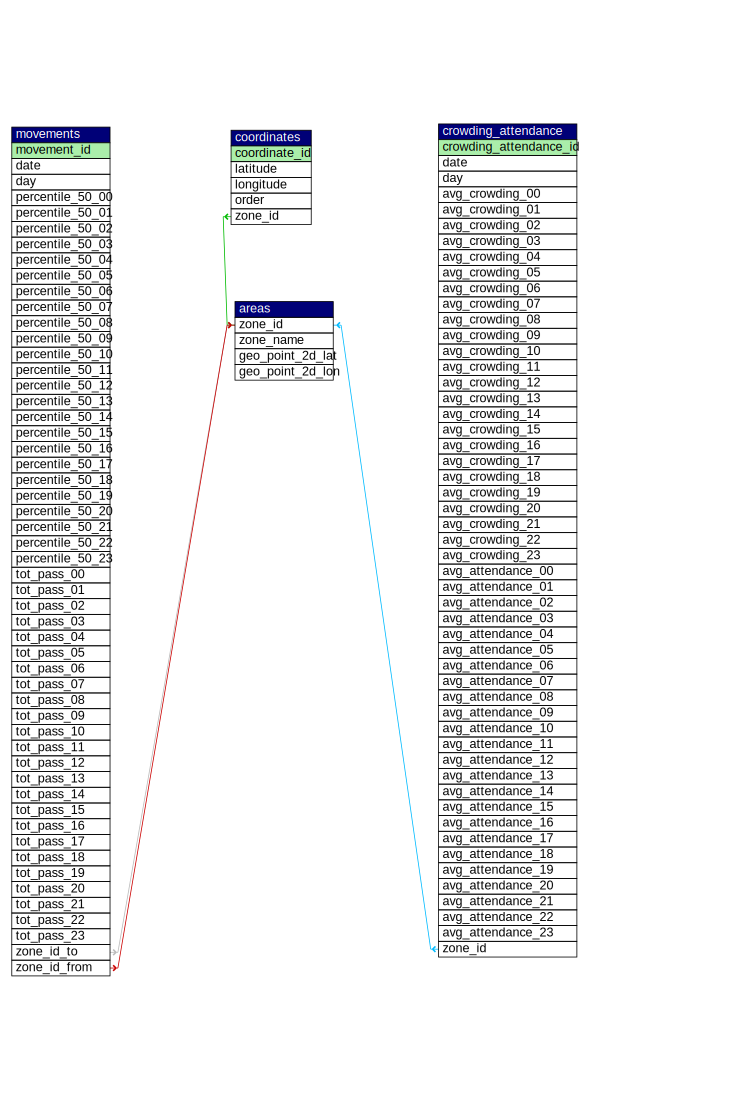
\includegraphics[width=\textwidth]{database.png}
    \caption[Schema del database]{Schema del database di BolognaWiFiMap. Notare la lista di attributi definiti per ciascuna ora.}
    \label{fig:database}
\end{figure}

\section{Connessione tra frontend e backend}
Dopo aver installato Vue.js e creato il progetto utilizzando Vite, ovvero un plugin di Vue per la nuova sintassi SFC (Single-File Components), abbiamo impostato l'indirizzo e la porta del server nel file di configurazione \Verb_vite.config.js_, settandolo a 0.0.0.0 per permettere al frontend di comunicare col backend indipendentemente dall'indirizzo del server, che in questo caso si riferisce a quello del server Apache. Inoltre, abbiamo specificato l'alias \Verb_@_ per definire la directory \Verb_./src/frontend_, semplificando il percorso dei file da importare.

\begin{figure}[H]
    \centering
    \includegraphics[width=\textwidth]{vite_config}
    \caption[Configurazione delle impostazioni Vite]{Configurazione delle impostazioni Vite relative al progetto Vue, dove si definiscono in particolare l'indirizzo e la porta per accedere al server.}
    \label{fig:vite_config}
\end{figure}

\section{Single-Page App}
Questa applicazione è stata realizzata seguendo il modello della \textit{Single-Page App}, ovvero una sola pagina web che carica selettivamente i suoi componenti o aggiorna i suoi dati senza necessità di ricaricare la pagina. Questo è permesso sia dallo stesso framework Vue.js, sia dall'implementazione di richieste AJAX che il client effettua al server.

\section{Implementazione richieste AJAX}
Le richieste AJAX sono effettuate in modo asincrono dal client al server per ottenere dei dati che verranno utilizzati per aggiornare la pagina, evitando di dover effettuare un ricaricamento della stessa. Per la sua implementazione abbiamo utilizzato la funzione \Verb_fetch()_ built-in di JavaScript, creando tre funzioni per aggiornare rispettivamente le aree, con \Verb_fetchAreas()_, gli spostamenti, con \Verb_fetchMovements()_, e infine l'affollamento insieme all'affluenza, con \Verb_fetchCrowdingAttendance()_. 

Abbiamo definito tutte queste funzioni nel file \Verb_api.js_, essendo molto semplici riportiamo in Figura~\ref{fig:ajax_api_movements} solo quella relativa agli spostamenti. In particolare, queste custom API utilizzano l'indirizzo corrente comprensivo di porta, per poi appendere a tale stringa l'url specifico dell'API a cui si vuole effettuare la richiesta. Si noti come questo setup presuppone un deployment di frontend e backend sullo stesso server, o quantomeno di un ridirezionamento tramite proxy di tali richieste effettuate a frontend verso l'url appropriato del backend, se dovessero essere in deployment su server diversi.

\begin{figure}[H]
    \centering
    \includegraphics[width=\textwidth]{ajax_api_movements}
    \caption[Funzione AJAX per ottenere la lista dei movimenti di una specifica data]{Implementazione di una funzione che effettua una richiesta AJAX per ottenere la lista dei movimenti di una specifica data.}
    \label{fig:ajax_api_movements}
\end{figure}

\section{Popolamento del database}
Affinché le richieste AJAX possano andare a buon fine, bisogna aver popolato il database. Questo compito è svolto mediante l'esecuzione del file \Verb_updater.php_, il quale controlla l'ultima data dei dati raccolti sul database e provvede ad aggiornarli, scaricando tutti i nuovi dati.

In fase di development o test, questo script viene lanciato manualmente, ma in un futuro deployment basterebbe automatizzare la sua esecuzione utilizzando Task Scheduler su Windows o un Cron Job su Linux. Tale script, riportato in Figura~\ref{fig:updater} richiama 3 funzioni differenti per svolgere il suo compito, che qui non mostreremo per via della loro lunghezza.

\begin{figure}[H]
    \centering
    \includegraphics[width=\textwidth]{updater_noligature}
    \caption[]{Script che viene eseguito per effettuare il setup o per aggiornare i dati sul database, utilizzando gli url definiti in \textit{urls.json} per effettuare le chiamate alle API del sito degli Open Data di BolognaWiFi \cite{BolognaWiFi_Spostamenti,BolognaWiFi_Affollamento,BolognaWiFi_Affluenza}.}
    \label{fig:updater}
\end{figure}

Innanzitutto, viene aggiornata la lista delle aree, nel caso se ne trovino di nuove. Quindi si scaricano, in ordine, prima i movimenti, poi l'affollamento insieme all'affluenza. All'interno di entrambe le funzioni, vengono scaricati i dati giorno per giorno, fino ad arrivare agli ultimi disponibili. Tuttavia, date le limitazioni delle API offerte da BolognaWiFi, vengono scaricati al massimo 100 elementi alla volta. Questo chunk così ottenuto viene messo in coda in una lista, per poi effettuare una nuova chiamata alla stessa API riguardante lo stesso giorno, ma con un offset aumentato di 100. Le stesse API pongono un limite totale di 10~100 alla somma di offset e numero di elementi, ma considerando che in un singolo giorno non si arriva nemmeno a 2~000 elementi totali in tutti e tre i dataset, tale limite effettivo di 10~000 all'offset non è poi così restrittivo.

% \section{Funzionalità}
\section{Informazioni su una zona o spostamento}
\section{Calcolo del colore di una zona}
\section{Raggruppamento dei dati giornalieri}
\section{Questionario SUS sull'esperienza utente}

\clearpage{\pagestyle{empty}\cleardoublepage}

\chapter*{Conclusioni}

\rhead[\fancyplain{}{\bfseries
CONCLUSIONI}]{\fancyplain{}{\bfseries\thepage}}
\lhead[\fancyplain{}{\bfseries\thepage}]{\fancyplain{}{\bfseries
CONCLUSIONI}}

\addcontentsline{toc}{chapter}{Conclusioni}

Questa tesi ha esplorato le potenzialità degli Open Data nella gestione e ottimizzazione dei servizi urbani, con particolare attenzione alla rete BolognaWiFi. L'obiettivo del progetto consisteva nello sviluppo di un'applicazione web interattiva per la visualizzazione dei dati relativi all'utilizzo della rete Wi-Fi pubblica del Comune di Bologna. Attraverso la creazione di un'interfaccia intuitiva e dinamica, è stato possibile rendere accessibili e interpretabili le informazioni raccolte, fornendo uno strumento utile per amministratori pubblici, ricercatori e cittadini.

Questa visualizzazione ha permesso di individuare a colpo d'occhio tendenze significative nell'utilizzo della rete, evidenziando pattern di affluenza, affollamento e spostamenti. La rappresentazione grafica di queste informazioni si è rivelata essenziale per facilitare la comprensione e l'elaborazione di strategie di miglioramento della connettività urbana. L'adozione di tecnologie moderne come Vue.js e Leaflet ha garantito un'interfaccia interattiva e altamente performante, migliorando l'esperienza utente e rendendo la navigazione più fluida ed efficace.

Il lavoro svolto ha dimostrato come l'uso intelligente degli Open Data possa migliorare significativamente la gestione e la pianificazione urbana. L'integrazione di strumenti di visualizzazione avanzati consente di sfruttare al meglio il potenziale dei dati pubblici, offrendo benefici concreti per la collettività. Grazie a questo progetto, è stato possibile non solo facilitare l'accesso alle informazioni sulla rete BolognaWiFi, ma anche proporre un modello replicabile per altre realtà urbane interessate alla valorizzazione dei propri dati.

Pur avendo raggiunto gli obiettivi prefissati, il progetto potrebbe essere ulteriormente ampliato e migliorato sotto diversi aspetti. Innanzitutto potremmo raffinare l'interfaccia utente, aggiungendo un grafico relativo all'andamento giornaliero, mensile o annuale, che per affollamento e affluenza sarebbe relativo a una singola zona, mentre per gli spostamenti, siano essi totali o mediani, andrebbe considerato un singolo movimento direzionato da una certa area verso un'altra. Riguardo agli spostamenti, si potrebbe calcolare il flusso in entrata e in uscita per ciascuna zona, assegnando dei relativi colori in scala cromatica per ogni area invece dell'attuale tinta monocromatica.

Inoltre, è importante notare come l'applicazione da noi creata permetta già adesso una possibile estensione ad altre città, aggiungendo i relativi dati sul database e modificando le coordinate iniziali della visualizzazione su mappa. L'unica vera esigenza sarebbe quella di adattare le API attuali per raccogliere i dati da una nuova banca dati di Open Data relativi alla città in cui si vuole estendere il servizio.

L'adozione di queste migliorie potrebbe trasformare l'applicazione sviluppata in un riferimento per la gestione e l'analisi dei dati urbani, promuovendo un uso più consapevole ed efficace delle risorse digitali a disposizione delle città. In questo modo potrebbe costituire un punto di partenza per ulteriori sviluppi nell'ambito della gestione delle infrastrutture digitali delle Smart Cities, contribuendo a rendere le città più connesse, intelligenti e a misura di cittadino.
%\clearpage{\pagestyle{empty}\cleardoublepage}

\cleardoublepage

\rhead[\fancyplain{}{\bfseries BIBLIOGRAFIA}]{\fancyplain{}{\bfseries\thepage}}
\lhead[\fancyplain{}{\bfseries\thepage}]{\fancyplain{}{\bfseries BIBLIOGRAFIA}}

\phantomsection % Enables an unnamed section to be referenced correctly in the table of contents
\addcontentsline{toc}{chapter}{Bibliografia}

% \renewcommand{\bibname}{Bibliografia} % Change title of bibliography for article class, use {\bibname} for report or book class, use {\refname} for article class
% \newpage
\bibliography{back/biblio}{}

%\bibliographystyle{unsrt}
\bibliographystyle{unsrtnat}

% \bibliographystyle{plainurl} % Use unsrturl to display an unsorted list

\rhead[\fancyplain{}{\bfseries \leftmark}]{\fancyplain{}{\bfseries
\thepage}}

\clearpage{\pagestyle{empty}\cleardoublepage}
\chapter*{Ringraziamenti}
\thispagestyle{empty}

\addcontentsline{toc}{chapter}{Ringraziamenti}

% Qui possiamo ringraziare il mondo intero!!!!!!!!!!\\
% Ovviamente solo se uno vuole, non \`e obbligatorio.

Vorrei ringraziare tutte le persone che mi hanno \sout{sopportato} supportato in questi anni, in particolare i miei amici e la mia famiglia, sempre rimasti vicini durante alti e bassi. Momenti che non sono certo mancati lungo questo percorso, grazie ai quali ho scoperto di avere al mio fianco delle persone vere, capaci di farti sentire a casa, fino al punto di rendere talvolta difficile congedarsi. E questo lo considero un grande privilegio.

Un sentito grazie va ai miei genitori, che mi hanno sempre incoraggiato a raggiungere i miei obiettivi e hanno contribuito a rendermi la persona che sono oggi. Si sono dimostrati molto più forti di quanto mi aspettassi, e non solo perché mi hanno sopportato quando studiavo in sessione. Vederli trovare il coraggio di andare avanti davvero non ha prezzo.

Ci tengo a nominare mia sorella, che mi ha sempre ricordato di non passare tutto il tempo sui libri, ma di ritagliarmi dei momenti di svago e coltivare i miei interessi. Senza saperlo è stata una vera maestra di vita, e la sua grinta continua a ispirarmi ogni giorno. Mi manchi tanto Annina.

Sento infine il bisogno di ringraziare alcuni amici speciali, senza fare nomi. Chi è riuscito a strapparmi un sorriso persino nelle giornate più nere. Chi mi è stato accanto e continua a offrire un supporto sicuro. Chi riesce a ispirarmi semplicemente essendo se stesso. Chi sa essere un comico tanto quanto un filosofo, con un pizzico di follia. Coloro che sono diventati letteralmente i fratelli di cui avevo bisogno, proprio al momento giusto. E infine, grazie a chi ha condiviso con me risate e momenti spensierati, perché alla fine sono questi i ricordi che contano davvero. Altro che quei banalissimi CFU.



\nocite{*}

%\cleardoublepage

%\listoffigures
%\listoftables


\end{document}
